% lecture4.tex -- GENERATED by build_L4.py from L4_numbers.json; do not edit by hand.
\documentclass[10pt,aspectratio=169,t]{beamer}
% =============================================================================
% nn_preamble.tex -- shared Beamer preamble of Neural Networks and Deep Learning (NN)
% Used by every lecture: lectures/Lk/lecturek.tex does
%   \documentclass[10pt,aspectratio=169,t]{beamer}
%   % =============================================================================
% nn_preamble.tex -- shared Beamer preamble of Neural Networks and Deep Learning (NN)
% Used by every lecture: lectures/Lk/lecturek.tex does
%   \documentclass[10pt,aspectratio=169,t]{beamer}
%   % =============================================================================
% nn_preamble.tex -- shared Beamer preamble of Neural Networks and Deep Learning (NN)
% Used by every lecture: lectures/Lk/lecturek.tex does
%   \documentclass[10pt,aspectratio=169,t]{beamer}
%   \input{../common/nn_preamble}
%   \nnlecture{k}{Lecture title}
% Logos live in lectures/common/logos/, charts in lectures/Lk/charts/.
% Do NOT add \hfuzz / \vfuzz / \hbadness here: overfull boxes must be fixed, not hidden.
% =============================================================================

\usetheme{default}
\setbeamersize{text margin left=7mm, text margin right=7mm}

% ---------------------------------------------------------------- packages
\usepackage[utf8]{inputenc}
\usepackage[T1]{fontenc}
\usepackage{lmodern}
\usepackage{amsmath, amssymb}
\usepackage{mathtools}
\usepackage{bm}
\usepackage{tikz}
\usetikzlibrary{arrows.meta, positioning, calc, shapes.misc}
\usepackage{booktabs}
\usepackage{array}
\usepackage{graphicx}
\usepackage{colortbl}
\usepackage{xcolor}
\usepackage{multicol}
\hypersetup{colorlinks=true, linkcolor=MainBlue, urlcolor=MainBlue, citecolor=MainBlue}
\graphicspath{{../common/logos/}}   % charts are included with their language folder: charts/en/, charts/ro/

% ---------------------------------------------------------------- colours
\definecolor{MainBlue}{RGB}{26, 58, 110}
\definecolor{IDAred}{RGB}{205, 0, 0}
\definecolor{DarkGray}{RGB}{51, 51, 51}
\definecolor{FooterGray}{RGB}{100, 100, 100}
\definecolor{BlockGray}{RGB}{236, 238, 242}
\definecolor{KeynoteGray}{RGB}{218, 218, 218}
\definecolor{Crimson}{RGB}{190, 40, 50}
\definecolor{Forest}{RGB}{30, 110, 50}
\definecolor{Bitter}{RGB}{214, 150, 20}
% chart palette (same hex values and order as lectures/common/nn_plot.py SERIES)
\definecolor{Ser1}{HTML}{2A78D6}
\definecolor{Ser2}{HTML}{EB6834}
\definecolor{Ser3}{HTML}{1BAF7A}
\definecolor{Ser4}{HTML}{EDA100}
\definecolor{Ser5}{HTML}{E87BA4}
\definecolor{Ser6}{HTML}{008300}
\definecolor{Ser7}{HTML}{6250D6}
\definecolor{Ser8}{HTML}{E34948}

\setbeamertemplate{background}{%
  \begin{tikzpicture}[remember picture, overlay]
    \shade[shading=axis, shading angle=315, top color=white, bottom color=KeynoteGray]
      (current page.south west) rectangle (current page.north east);
  \end{tikzpicture}}
\setbeamercolor{background canvas}{bg=}
\setbeamercolor{structure}{fg=MainBlue}
\setbeamercolor{normal text}{fg=DarkGray}
\setbeamercolor{title}{fg=IDAred}
\setbeamercolor{frametitle}{fg=IDAred, bg=}
\setbeamercolor{block title}{bg=MainBlue, fg=white}
\setbeamercolor{block body}{bg=BlockGray, fg=DarkGray}
\setbeamercolor{block title alerted}{bg=Crimson, fg=white}
\setbeamercolor{block body alerted}{bg=Crimson!7, fg=DarkGray}
\setbeamercolor{block title example}{bg=Forest, fg=white}
\setbeamercolor{block body example}{bg=Forest!7, fg=DarkGray}
\setbeamercolor{item}{fg=MainBlue}
\setbeamerfont{frametitle}{size=\large, series=\bfseries}
\setbeamerfont{block title}{size=\small, series=\bfseries}
\setbeamertemplate{blocks}[rounded][shadow=false]
\setbeamertemplate{itemize item}{\color{MainBlue}$\boxdot$}
\setbeamertemplate{itemize subitem}{\color{MainBlue}\scriptsize$\blacktriangleright$}
% compact two-level lists: level 1 = main point, level 2 = details (no text outside bullets)
\setbeamerfont{itemize/enumerate subbody}{size=\footnotesize}
\setlength{\leftmargini}{1.1em}
\setlength{\leftmarginii}{1.1em}
\setbeamertemplate{itemize/enumerate body begin}{\setlength{\topsep}{0pt}\setlength{\partopsep}{0pt}\setlength{\parskip}{0pt}}
\setbeamertemplate{itemize/enumerate subbody begin}{\setlength{\topsep}{0pt}\setlength{\partopsep}{0pt}\setlength{\itemsep}{0pt}\vspace{-0.4ex}}

\setbeamertemplate{enumerate item}{\color{MainBlue}\insertenumlabel.}
\setlength{\leftmargini}{1.3em}
\setlength{\leftmarginii}{1.2em}
\setbeamertemplate{navigation symbols}{}
\setbeamertemplate{section in toc}{\color{MainBlue}$\blacktriangleright$~\inserttocsection}
\setbeamertemplate{caption}{\raggedright\insertcaption\par}
% frame subtitle = precise citation line under the claim title (Weron style)
\setbeamerfont{framesubtitle}{size=\footnotesize}
\setbeamercolor{framesubtitle}{fg=FooterGray}
% outline that reappears at every section with the current section highlighted
\setbeamertemplate{section in toc shaded}[default][35]
\setbeamertemplate{subsection in toc shaded}[default][35]
\setbeamertemplate{subsection in toc}{\leavevmode\leftskip=2.2em\color{DarkGray}\small\inserttocsubsection\par}
\AtBeginSection[]{{\begin{frame}{\txtoutline}\vspace{2mm}\small
  \tableofcontents[currentsection,hideothersubsections]\end{frame}}}

% ---------------------------------------------------------------- head and foot
\setbeamertemplate{headline}{%
  \vskip10pt%
  \hbox to \paperwidth{\hskip0.5cm%
    {\small\color{FooterGray}\renewcommand{\hyperlink}[2]{##2}\insertsectionhead}%
    \hfill\textcolor{FooterGray}{\small\insertframenumber}\hskip0.5cm}%
  \vskip4pt{\color{FooterGray}\hrule height 0.4pt}}
% footer as in the other courses (MFM, SFM): course name on the left, small sparkline on the right
\setbeamertemplate{footline}{%
  {\color{FooterGray}\hrule height 0.4pt}\vskip4pt%
  \hbox to \paperwidth{\hskip0.5cm%
    \textcolor{FooterGray}{\small\txtcourse}%
    \hfill\raisebox{-0.1em}{\begin{tikzpicture}[x=0.08em, y=0.08em, line width=0.4pt]
      \draw[FooterGray] (0,3) -- (1,4) -- (2,3.5) -- (3,5) -- (4,4) -- (5,6) -- (6,5.5) -- (7,4) -- (8,5) -- (9,7) -- (10,6) -- (11,5) -- (12,6.5) -- (13,8) -- (14,7) -- (15,6) -- (16,7.5) -- (17,9) -- (18,8) -- (19,7) -- (20,8.5) -- (21,10) -- (22,9) -- (23,8) -- (24,9.5);
    \end{tikzpicture}}\hskip0.5cm}%
  \vskip6pt}

% ---------------------------------------------------------------- title page
\defbeamertemplate*{title page}{nn}[1][]{%
  \vspace{0.15cm}
  \begin{center}
    \href{https://www.ase.ro}{
\includegraphics[height=0.9cm]{ase_logo.png}}\hspace{0.3cm}%
    \href{https://ipe.ro/new}{
\includegraphics[height=0.9cm]{acad_logo.png}}\hspace{0.3cm}%
    \href{https://theida.net}{
\includegraphics[height=0.9cm]{ida_logo.png}}\hspace{0.3cm}%
    \href{https://blockchain-research-center.com}{
\includegraphics[height=0.9cm]{brc_logo.png}}\hspace{0.3cm}%
    \href{https://www.ai4efin.ase.ro}{
\includegraphics[height=0.9cm]{ai4efin_logo.png}}\hspace{0.3cm}%
    \href{https://www.digital-finance-msca.com}{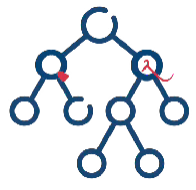
\includegraphics[height=0.9cm]{msca_logo.png}}%
  \end{center}
  \vspace{0.45cm}
  \begin{center}
    \begin{minipage}{0.1\textwidth}\centering
      \href{https://quantlet.com}{
\includegraphics[height=0.9cm]{ql_logo.png}}\end{minipage}%
    \begin{minipage}{0.78\textwidth}\centering
      {\Large\bfseries\usebeamercolor[fg]{title}\inserttitle}\par\vspace{0.25cm}
      {\large\usebeamercolor[fg]{title}\insertsubtitle}\end{minipage}%
    \begin{minipage}{0.1\textwidth}\centering
      \href{https://quantinar.com}{
\includegraphics[height=0.9cm]{qr_logo.png}}\end{minipage}
  \end{center}
  \vfill
  \hspace{0.4cm}{\bfseries\insertauthor}\par\vspace{0.12cm}
  \hspace{0.4cm}\begin{minipage}[t]{0.92\textwidth}\raggedright\footnotesize\insertinstitute\end{minipage}
  \par\vspace{0.4cm}}

% ---------------------------------------------------------------- lecture metadata
\newcommand{\nnshort}{}
\newcommand{\nnnb}{notebooks}
\newcommand{\nnrepo}{https://github.com/danpele/NEURAL_BIZ/tree/main}
% language-dependent labels (English default; \nnromanian switches to Romanian, call it before \nnlecture)
\newcommand{\txtcourse}{Neural Networks and Deep Learning}
\newcommand{\txtlecture}{Lecture}
\newcommand{\txtoutline}{Outline}
\newcommand{\txtintuition}{In one sentence:}
\newcommand{\txtjob}{In practice:}
\newcommand{\txttry}{Experiment yourself:}
\newcommand{\txtwhere}{where}
\newcommand{\txtsim}{SIMULATED DATA (teaching illustration)}
\newcommand{\txtnbsuffix}{}
\newcommand{\txtinstitute}{Bucharest University of Economic Studies (ASE), Department of Statistics and Econometrics\\
    Romanian Academy, Institute for Economic Forecasting (IPE)\\
    IDA Institute Digital Assets \textbullet\ AI4EFin \textbullet\ MSCA Digital Finance}
\newcommand{\nnromanian}{%
  \renewcommand{\txtcourse}{Rețele neuronale și deep learning}%
  \renewcommand{\txtlecture}{Cursul}%
  \renewcommand{\txtoutline}{Cuprins}%
  \renewcommand{\txtintuition}{Pe scurt:}%
  \renewcommand{\txtjob}{În practică:}%
  \renewcommand{\txttry}{Exercițiu practic:}%
  \renewcommand{\txtwhere}{unde}%
  \renewcommand{\txtsim}{DATE SIMULATE (doar pentru ilustrare)}%
  \renewcommand{\txtnbsuffix}{\string_ro}%
  \renewcommand{\txtinstitute}{Academia de Studii Economice din București (ASE), Departamentul de Statistică și Econometrie\\
    Academia Română, Institutul de Prognoză Economică (IPE)\\
    IDA Institute Digital Assets \textbullet\ AI4EFin \textbullet\ MSCA Digital Finance}}
\newcommand{\nnlecture}[2]{%
  \renewcommand{\nnshort}{\txtlecture\ #1}%
  \renewcommand{\nnnb}{notebooks/L#1\string_notebook\txtnbsuffix.ipynb}%
  \title[NN]{\txtcourse}%
  \subtitle{\txtlecture\ #1: #2}%
  \author{Prof.\ dr.\ Daniel Traian PELE}%
  \institute{\txtinstitute}%
  \date{}}

% ---------------------------------------------------------------- teaching blocks (one message per frame)
% \intuition{one plain sentence}  ->  formula with every symbol defined  ->  real-data example  ->  \manager{one line}
\newcommand{\intuition}[1]{\begin{itemize}\item {\color{MainBlue}\textbf{\txtintuition}}~#1\end{itemize}\vspace{0.6mm}}
\newcommand{\manager}[1]{\colorbox{Forest!10}{\parbox{\dimexpr\linewidth-2\fboxsep\relax}{\footnotesize
  \begin{itemize}\setlength{\itemsep}{0pt}\item \textbf{\color{Forest}\txtjob}~#1\end{itemize}}}}
% Experiment yourself: pointer to the matching notebook section
\newcommand{\tryit}[1]{{\scriptsize\href{\nnrepo/\nnnb}{%
  \raisebox{-0.15em}{
\includegraphics[height=0.85em]{ql_logo.png}}\,\textbf{\txttry}~\color{MainBlue}#1}}}
% bottom row: manager line (left) + experiment pointer (right), pinned to the bottom of the frame
\newcommand{\bottomrow}[2]{\par\vfill\noindent\begin{minipage}[b]{0.72\linewidth}#1\end{minipage}\hfill
  \begin{minipage}[b]{0.26\linewidth}\raggedleft #2\end{minipage}\par\vspace{0.5mm}}
\newcommand{\where}[1]{{\footnotesize\textbf{\txtwhere}~#1\par}}

% ---------------------------------------------------------------- helpers
% chart source line under a figure: \chartsource{Source ...; period ...}
\newcommand{\chartsource}[1]{\par\vspace{1pt}{\scriptsize\color{FooterGray}#1\par}}
% link to code: \quantlet{label}{path inside the repo}
\newcommand{\quantlet}[2]{\par\vspace{1pt}\hfill\href{\nnrepo/#2}{%
  \raisebox{-0.15em}{
\includegraphics[height=0.75em]{ql_logo.png}}\textcolor{MainBlue}{\scriptsize\ #1}}}
% inline Quantlet link for the bottom-right corner of a frame: \qlink{label}{path inside the repo}
\newcommand{\qlink}[2]{{\scriptsize\href{\nnrepo/#2}{\raisebox{-0.15em}{
\includegraphics[height=0.85em]{ql_logo.png}}\,\textcolor{MainBlue}{#1}}}}
\newcommand{\simlabel}{\colorbox{Crimson!12}{\scriptsize\bfseries\color{Crimson}\txtsim}}
\newcommand{\E}{\mathbb{E}}
\newcommand{\Var}{\operatorname{Var}}
\newcommand{\Cov}{\operatorname{Cov}}
\newcommand{\Corr}{\operatorname{Corr}}
\newcommand{\asinh}{\operatorname{asinh}}
\newcommand{\iid}{\overset{\text{i.i.d.}}{\sim}}
\newcommand{\EUR}{EUR}
% deep-learning notation (Bishop & Bishop, 2024): vectors bold lower case, matrices bold upper case
\newcommand{\R}{\mathbb{R}}
\newcommand{\vx}{\mathbf{x}}
\newcommand{\vy}{\mathbf{y}}
\newcommand{\vz}{\mathbf{z}}
\newcommand{\vh}{\mathbf{h}}
\newcommand{\vw}{\mathbf{w}}
\newcommand{\vb}{\mathbf{b}}
\newcommand{\mW}{\mathbf{W}}
\newcommand{\mX}{\mathbf{X}}
\newcommand{\btheta}{\boldsymbol{\theta}}
\newcommand{\loss}{\mathcal{L}}
\newcommand{\dataset}{\mathcal{D}}
\DeclareMathOperator*{\argmin}{arg\,min}
\DeclareMathOperator*{\argmax}{arg\,max}
\DeclareMathOperator{\softmax}{softmax}
\DeclareMathOperator{\ReLU}{ReLU}
\DeclareMathOperator{\sigm}{\sigma}

%   \nnlecture{k}{Lecture title}
% Logos live in lectures/common/logos/, charts in lectures/Lk/charts/.
% Do NOT add \hfuzz / \vfuzz / \hbadness here: overfull boxes must be fixed, not hidden.
% =============================================================================

\usetheme{default}
\setbeamersize{text margin left=7mm, text margin right=7mm}

% ---------------------------------------------------------------- packages
\usepackage[utf8]{inputenc}
\usepackage[T1]{fontenc}
\usepackage{lmodern}
\usepackage{amsmath, amssymb}
\usepackage{mathtools}
\usepackage{bm}
\usepackage{tikz}
\usetikzlibrary{arrows.meta, positioning, calc, shapes.misc}
\usepackage{booktabs}
\usepackage{array}
\usepackage{graphicx}
\usepackage{colortbl}
\usepackage{xcolor}
\usepackage{multicol}
\hypersetup{colorlinks=true, linkcolor=MainBlue, urlcolor=MainBlue, citecolor=MainBlue}
\graphicspath{{../common/logos/}}   % charts are included with their language folder: charts/en/, charts/ro/

% ---------------------------------------------------------------- colours
\definecolor{MainBlue}{RGB}{26, 58, 110}
\definecolor{IDAred}{RGB}{205, 0, 0}
\definecolor{DarkGray}{RGB}{51, 51, 51}
\definecolor{FooterGray}{RGB}{100, 100, 100}
\definecolor{BlockGray}{RGB}{236, 238, 242}
\definecolor{KeynoteGray}{RGB}{218, 218, 218}
\definecolor{Crimson}{RGB}{190, 40, 50}
\definecolor{Forest}{RGB}{30, 110, 50}
\definecolor{Bitter}{RGB}{214, 150, 20}
% chart palette (same hex values and order as lectures/common/nn_plot.py SERIES)
\definecolor{Ser1}{HTML}{2A78D6}
\definecolor{Ser2}{HTML}{EB6834}
\definecolor{Ser3}{HTML}{1BAF7A}
\definecolor{Ser4}{HTML}{EDA100}
\definecolor{Ser5}{HTML}{E87BA4}
\definecolor{Ser6}{HTML}{008300}
\definecolor{Ser7}{HTML}{6250D6}
\definecolor{Ser8}{HTML}{E34948}

\setbeamertemplate{background}{%
  \begin{tikzpicture}[remember picture, overlay]
    \shade[shading=axis, shading angle=315, top color=white, bottom color=KeynoteGray]
      (current page.south west) rectangle (current page.north east);
  \end{tikzpicture}}
\setbeamercolor{background canvas}{bg=}
\setbeamercolor{structure}{fg=MainBlue}
\setbeamercolor{normal text}{fg=DarkGray}
\setbeamercolor{title}{fg=IDAred}
\setbeamercolor{frametitle}{fg=IDAred, bg=}
\setbeamercolor{block title}{bg=MainBlue, fg=white}
\setbeamercolor{block body}{bg=BlockGray, fg=DarkGray}
\setbeamercolor{block title alerted}{bg=Crimson, fg=white}
\setbeamercolor{block body alerted}{bg=Crimson!7, fg=DarkGray}
\setbeamercolor{block title example}{bg=Forest, fg=white}
\setbeamercolor{block body example}{bg=Forest!7, fg=DarkGray}
\setbeamercolor{item}{fg=MainBlue}
\setbeamerfont{frametitle}{size=\large, series=\bfseries}
\setbeamerfont{block title}{size=\small, series=\bfseries}
\setbeamertemplate{blocks}[rounded][shadow=false]
\setbeamertemplate{itemize item}{\color{MainBlue}$\boxdot$}
\setbeamertemplate{itemize subitem}{\color{MainBlue}\scriptsize$\blacktriangleright$}
% compact two-level lists: level 1 = main point, level 2 = details (no text outside bullets)
\setbeamerfont{itemize/enumerate subbody}{size=\footnotesize}
\setlength{\leftmargini}{1.1em}
\setlength{\leftmarginii}{1.1em}
\setbeamertemplate{itemize/enumerate body begin}{\setlength{\topsep}{0pt}\setlength{\partopsep}{0pt}\setlength{\parskip}{0pt}}
\setbeamertemplate{itemize/enumerate subbody begin}{\setlength{\topsep}{0pt}\setlength{\partopsep}{0pt}\setlength{\itemsep}{0pt}\vspace{-0.4ex}}

\setbeamertemplate{enumerate item}{\color{MainBlue}\insertenumlabel.}
\setlength{\leftmargini}{1.3em}
\setlength{\leftmarginii}{1.2em}
\setbeamertemplate{navigation symbols}{}
\setbeamertemplate{section in toc}{\color{MainBlue}$\blacktriangleright$~\inserttocsection}
\setbeamertemplate{caption}{\raggedright\insertcaption\par}
% frame subtitle = precise citation line under the claim title (Weron style)
\setbeamerfont{framesubtitle}{size=\footnotesize}
\setbeamercolor{framesubtitle}{fg=FooterGray}
% outline that reappears at every section with the current section highlighted
\setbeamertemplate{section in toc shaded}[default][35]
\setbeamertemplate{subsection in toc shaded}[default][35]
\setbeamertemplate{subsection in toc}{\leavevmode\leftskip=2.2em\color{DarkGray}\small\inserttocsubsection\par}
\AtBeginSection[]{{\begin{frame}{\txtoutline}\vspace{2mm}\small
  \tableofcontents[currentsection,hideothersubsections]\end{frame}}}

% ---------------------------------------------------------------- head and foot
\setbeamertemplate{headline}{%
  \vskip10pt%
  \hbox to \paperwidth{\hskip0.5cm%
    {\small\color{FooterGray}\renewcommand{\hyperlink}[2]{##2}\insertsectionhead}%
    \hfill\textcolor{FooterGray}{\small\insertframenumber}\hskip0.5cm}%
  \vskip4pt{\color{FooterGray}\hrule height 0.4pt}}
% footer as in the other courses (MFM, SFM): course name on the left, small sparkline on the right
\setbeamertemplate{footline}{%
  {\color{FooterGray}\hrule height 0.4pt}\vskip4pt%
  \hbox to \paperwidth{\hskip0.5cm%
    \textcolor{FooterGray}{\small\txtcourse}%
    \hfill\raisebox{-0.1em}{\begin{tikzpicture}[x=0.08em, y=0.08em, line width=0.4pt]
      \draw[FooterGray] (0,3) -- (1,4) -- (2,3.5) -- (3,5) -- (4,4) -- (5,6) -- (6,5.5) -- (7,4) -- (8,5) -- (9,7) -- (10,6) -- (11,5) -- (12,6.5) -- (13,8) -- (14,7) -- (15,6) -- (16,7.5) -- (17,9) -- (18,8) -- (19,7) -- (20,8.5) -- (21,10) -- (22,9) -- (23,8) -- (24,9.5);
    \end{tikzpicture}}\hskip0.5cm}%
  \vskip6pt}

% ---------------------------------------------------------------- title page
\defbeamertemplate*{title page}{nn}[1][]{%
  \vspace{0.15cm}
  \begin{center}
    \href{https://www.ase.ro}{
\includegraphics[height=0.9cm]{ase_logo.png}}\hspace{0.3cm}%
    \href{https://ipe.ro/new}{
\includegraphics[height=0.9cm]{acad_logo.png}}\hspace{0.3cm}%
    \href{https://theida.net}{
\includegraphics[height=0.9cm]{ida_logo.png}}\hspace{0.3cm}%
    \href{https://blockchain-research-center.com}{
\includegraphics[height=0.9cm]{brc_logo.png}}\hspace{0.3cm}%
    \href{https://www.ai4efin.ase.ro}{
\includegraphics[height=0.9cm]{ai4efin_logo.png}}\hspace{0.3cm}%
    \href{https://www.digital-finance-msca.com}{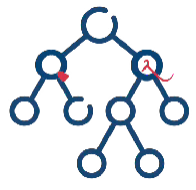
\includegraphics[height=0.9cm]{msca_logo.png}}%
  \end{center}
  \vspace{0.45cm}
  \begin{center}
    \begin{minipage}{0.1\textwidth}\centering
      \href{https://quantlet.com}{
\includegraphics[height=0.9cm]{ql_logo.png}}\end{minipage}%
    \begin{minipage}{0.78\textwidth}\centering
      {\Large\bfseries\usebeamercolor[fg]{title}\inserttitle}\par\vspace{0.25cm}
      {\large\usebeamercolor[fg]{title}\insertsubtitle}\end{minipage}%
    \begin{minipage}{0.1\textwidth}\centering
      \href{https://quantinar.com}{
\includegraphics[height=0.9cm]{qr_logo.png}}\end{minipage}
  \end{center}
  \vfill
  \hspace{0.4cm}{\bfseries\insertauthor}\par\vspace{0.12cm}
  \hspace{0.4cm}\begin{minipage}[t]{0.92\textwidth}\raggedright\footnotesize\insertinstitute\end{minipage}
  \par\vspace{0.4cm}}

% ---------------------------------------------------------------- lecture metadata
\newcommand{\nnshort}{}
\newcommand{\nnnb}{notebooks}
\newcommand{\nnrepo}{https://github.com/danpele/NEURAL_BIZ/tree/main}
% language-dependent labels (English default; \nnromanian switches to Romanian, call it before \nnlecture)
\newcommand{\txtcourse}{Neural Networks and Deep Learning}
\newcommand{\txtlecture}{Lecture}
\newcommand{\txtoutline}{Outline}
\newcommand{\txtintuition}{In one sentence:}
\newcommand{\txtjob}{In practice:}
\newcommand{\txttry}{Experiment yourself:}
\newcommand{\txtwhere}{where}
\newcommand{\txtsim}{SIMULATED DATA (teaching illustration)}
\newcommand{\txtnbsuffix}{}
\newcommand{\txtinstitute}{Bucharest University of Economic Studies (ASE), Department of Statistics and Econometrics\\
    Romanian Academy, Institute for Economic Forecasting (IPE)\\
    IDA Institute Digital Assets \textbullet\ AI4EFin \textbullet\ MSCA Digital Finance}
\newcommand{\nnromanian}{%
  \renewcommand{\txtcourse}{Rețele neuronale și deep learning}%
  \renewcommand{\txtlecture}{Cursul}%
  \renewcommand{\txtoutline}{Cuprins}%
  \renewcommand{\txtintuition}{Pe scurt:}%
  \renewcommand{\txtjob}{În practică:}%
  \renewcommand{\txttry}{Exercițiu practic:}%
  \renewcommand{\txtwhere}{unde}%
  \renewcommand{\txtsim}{DATE SIMULATE (doar pentru ilustrare)}%
  \renewcommand{\txtnbsuffix}{\string_ro}%
  \renewcommand{\txtinstitute}{Academia de Studii Economice din București (ASE), Departamentul de Statistică și Econometrie\\
    Academia Română, Institutul de Prognoză Economică (IPE)\\
    IDA Institute Digital Assets \textbullet\ AI4EFin \textbullet\ MSCA Digital Finance}}
\newcommand{\nnlecture}[2]{%
  \renewcommand{\nnshort}{\txtlecture\ #1}%
  \renewcommand{\nnnb}{notebooks/L#1\string_notebook\txtnbsuffix.ipynb}%
  \title[NN]{\txtcourse}%
  \subtitle{\txtlecture\ #1: #2}%
  \author{Prof.\ dr.\ Daniel Traian PELE}%
  \institute{\txtinstitute}%
  \date{}}

% ---------------------------------------------------------------- teaching blocks (one message per frame)
% \intuition{one plain sentence}  ->  formula with every symbol defined  ->  real-data example  ->  \manager{one line}
\newcommand{\intuition}[1]{\begin{itemize}\item {\color{MainBlue}\textbf{\txtintuition}}~#1\end{itemize}\vspace{0.6mm}}
\newcommand{\manager}[1]{\colorbox{Forest!10}{\parbox{\dimexpr\linewidth-2\fboxsep\relax}{\footnotesize
  \begin{itemize}\setlength{\itemsep}{0pt}\item \textbf{\color{Forest}\txtjob}~#1\end{itemize}}}}
% Experiment yourself: pointer to the matching notebook section
\newcommand{\tryit}[1]{{\scriptsize\href{\nnrepo/\nnnb}{%
  \raisebox{-0.15em}{
\includegraphics[height=0.85em]{ql_logo.png}}\,\textbf{\txttry}~\color{MainBlue}#1}}}
% bottom row: manager line (left) + experiment pointer (right), pinned to the bottom of the frame
\newcommand{\bottomrow}[2]{\par\vfill\noindent\begin{minipage}[b]{0.72\linewidth}#1\end{minipage}\hfill
  \begin{minipage}[b]{0.26\linewidth}\raggedleft #2\end{minipage}\par\vspace{0.5mm}}
\newcommand{\where}[1]{{\footnotesize\textbf{\txtwhere}~#1\par}}

% ---------------------------------------------------------------- helpers
% chart source line under a figure: \chartsource{Source ...; period ...}
\newcommand{\chartsource}[1]{\par\vspace{1pt}{\scriptsize\color{FooterGray}#1\par}}
% link to code: \quantlet{label}{path inside the repo}
\newcommand{\quantlet}[2]{\par\vspace{1pt}\hfill\href{\nnrepo/#2}{%
  \raisebox{-0.15em}{
\includegraphics[height=0.75em]{ql_logo.png}}\textcolor{MainBlue}{\scriptsize\ #1}}}
% inline Quantlet link for the bottom-right corner of a frame: \qlink{label}{path inside the repo}
\newcommand{\qlink}[2]{{\scriptsize\href{\nnrepo/#2}{\raisebox{-0.15em}{
\includegraphics[height=0.85em]{ql_logo.png}}\,\textcolor{MainBlue}{#1}}}}
\newcommand{\simlabel}{\colorbox{Crimson!12}{\scriptsize\bfseries\color{Crimson}\txtsim}}
\newcommand{\E}{\mathbb{E}}
\newcommand{\Var}{\operatorname{Var}}
\newcommand{\Cov}{\operatorname{Cov}}
\newcommand{\Corr}{\operatorname{Corr}}
\newcommand{\asinh}{\operatorname{asinh}}
\newcommand{\iid}{\overset{\text{i.i.d.}}{\sim}}
\newcommand{\EUR}{EUR}
% deep-learning notation (Bishop & Bishop, 2024): vectors bold lower case, matrices bold upper case
\newcommand{\R}{\mathbb{R}}
\newcommand{\vx}{\mathbf{x}}
\newcommand{\vy}{\mathbf{y}}
\newcommand{\vz}{\mathbf{z}}
\newcommand{\vh}{\mathbf{h}}
\newcommand{\vw}{\mathbf{w}}
\newcommand{\vb}{\mathbf{b}}
\newcommand{\mW}{\mathbf{W}}
\newcommand{\mX}{\mathbf{X}}
\newcommand{\btheta}{\boldsymbol{\theta}}
\newcommand{\loss}{\mathcal{L}}
\newcommand{\dataset}{\mathcal{D}}
\DeclareMathOperator*{\argmin}{arg\,min}
\DeclareMathOperator*{\argmax}{arg\,max}
\DeclareMathOperator{\softmax}{softmax}
\DeclareMathOperator{\ReLU}{ReLU}
\DeclareMathOperator{\sigm}{\sigma}

%   \nnlecture{k}{Lecture title}
% Logos live in lectures/common/logos/, charts in lectures/Lk/charts/.
% Do NOT add \hfuzz / \vfuzz / \hbadness here: overfull boxes must be fixed, not hidden.
% =============================================================================

\usetheme{default}
\setbeamersize{text margin left=7mm, text margin right=7mm}

% ---------------------------------------------------------------- packages
\usepackage[utf8]{inputenc}
\usepackage[T1]{fontenc}
\usepackage{lmodern}
\usepackage{amsmath, amssymb}
\usepackage{mathtools}
\usepackage{bm}
\usepackage{tikz}
\usetikzlibrary{arrows.meta, positioning, calc, shapes.misc}
\usepackage{booktabs}
\usepackage{array}
\usepackage{graphicx}
\usepackage{colortbl}
\usepackage{xcolor}
\usepackage{multicol}
\hypersetup{colorlinks=true, linkcolor=MainBlue, urlcolor=MainBlue, citecolor=MainBlue}
\graphicspath{{../common/logos/}}   % charts are included with their language folder: charts/en/, charts/ro/

% ---------------------------------------------------------------- colours
\definecolor{MainBlue}{RGB}{26, 58, 110}
\definecolor{IDAred}{RGB}{205, 0, 0}
\definecolor{DarkGray}{RGB}{51, 51, 51}
\definecolor{FooterGray}{RGB}{100, 100, 100}
\definecolor{BlockGray}{RGB}{236, 238, 242}
\definecolor{KeynoteGray}{RGB}{218, 218, 218}
\definecolor{Crimson}{RGB}{190, 40, 50}
\definecolor{Forest}{RGB}{30, 110, 50}
\definecolor{Bitter}{RGB}{214, 150, 20}
% chart palette (same hex values and order as lectures/common/nn_plot.py SERIES)
\definecolor{Ser1}{HTML}{2A78D6}
\definecolor{Ser2}{HTML}{EB6834}
\definecolor{Ser3}{HTML}{1BAF7A}
\definecolor{Ser4}{HTML}{EDA100}
\definecolor{Ser5}{HTML}{E87BA4}
\definecolor{Ser6}{HTML}{008300}
\definecolor{Ser7}{HTML}{6250D6}
\definecolor{Ser8}{HTML}{E34948}

\setbeamertemplate{background}{%
  \begin{tikzpicture}[remember picture, overlay]
    \shade[shading=axis, shading angle=315, top color=white, bottom color=KeynoteGray]
      (current page.south west) rectangle (current page.north east);
  \end{tikzpicture}}
\setbeamercolor{background canvas}{bg=}
\setbeamercolor{structure}{fg=MainBlue}
\setbeamercolor{normal text}{fg=DarkGray}
\setbeamercolor{title}{fg=IDAred}
\setbeamercolor{frametitle}{fg=IDAred, bg=}
\setbeamercolor{block title}{bg=MainBlue, fg=white}
\setbeamercolor{block body}{bg=BlockGray, fg=DarkGray}
\setbeamercolor{block title alerted}{bg=Crimson, fg=white}
\setbeamercolor{block body alerted}{bg=Crimson!7, fg=DarkGray}
\setbeamercolor{block title example}{bg=Forest, fg=white}
\setbeamercolor{block body example}{bg=Forest!7, fg=DarkGray}
\setbeamercolor{item}{fg=MainBlue}
\setbeamerfont{frametitle}{size=\large, series=\bfseries}
\setbeamerfont{block title}{size=\small, series=\bfseries}
\setbeamertemplate{blocks}[rounded][shadow=false]
\setbeamertemplate{itemize item}{\color{MainBlue}$\boxdot$}
\setbeamertemplate{itemize subitem}{\color{MainBlue}\scriptsize$\blacktriangleright$}
% compact two-level lists: level 1 = main point, level 2 = details (no text outside bullets)
\setbeamerfont{itemize/enumerate subbody}{size=\footnotesize}
\setlength{\leftmargini}{1.1em}
\setlength{\leftmarginii}{1.1em}
\setbeamertemplate{itemize/enumerate body begin}{\setlength{\topsep}{0pt}\setlength{\partopsep}{0pt}\setlength{\parskip}{0pt}}
\setbeamertemplate{itemize/enumerate subbody begin}{\setlength{\topsep}{0pt}\setlength{\partopsep}{0pt}\setlength{\itemsep}{0pt}\vspace{-0.4ex}}

\setbeamertemplate{enumerate item}{\color{MainBlue}\insertenumlabel.}
\setlength{\leftmargini}{1.3em}
\setlength{\leftmarginii}{1.2em}
\setbeamertemplate{navigation symbols}{}
\setbeamertemplate{section in toc}{\color{MainBlue}$\blacktriangleright$~\inserttocsection}
\setbeamertemplate{caption}{\raggedright\insertcaption\par}
% frame subtitle = precise citation line under the claim title (Weron style)
\setbeamerfont{framesubtitle}{size=\footnotesize}
\setbeamercolor{framesubtitle}{fg=FooterGray}
% outline that reappears at every section with the current section highlighted
\setbeamertemplate{section in toc shaded}[default][35]
\setbeamertemplate{subsection in toc shaded}[default][35]
\setbeamertemplate{subsection in toc}{\leavevmode\leftskip=2.2em\color{DarkGray}\small\inserttocsubsection\par}
\AtBeginSection[]{{\begin{frame}{\txtoutline}\vspace{2mm}\small
  \tableofcontents[currentsection,hideothersubsections]\end{frame}}}

% ---------------------------------------------------------------- head and foot
\setbeamertemplate{headline}{%
  \vskip10pt%
  \hbox to \paperwidth{\hskip0.5cm%
    {\small\color{FooterGray}\renewcommand{\hyperlink}[2]{##2}\insertsectionhead}%
    \hfill\textcolor{FooterGray}{\small\insertframenumber}\hskip0.5cm}%
  \vskip4pt{\color{FooterGray}\hrule height 0.4pt}}
% footer as in the other courses (MFM, SFM): course name on the left, small sparkline on the right
\setbeamertemplate{footline}{%
  {\color{FooterGray}\hrule height 0.4pt}\vskip4pt%
  \hbox to \paperwidth{\hskip0.5cm%
    \textcolor{FooterGray}{\small\txtcourse}%
    \hfill\raisebox{-0.1em}{\begin{tikzpicture}[x=0.08em, y=0.08em, line width=0.4pt]
      \draw[FooterGray] (0,3) -- (1,4) -- (2,3.5) -- (3,5) -- (4,4) -- (5,6) -- (6,5.5) -- (7,4) -- (8,5) -- (9,7) -- (10,6) -- (11,5) -- (12,6.5) -- (13,8) -- (14,7) -- (15,6) -- (16,7.5) -- (17,9) -- (18,8) -- (19,7) -- (20,8.5) -- (21,10) -- (22,9) -- (23,8) -- (24,9.5);
    \end{tikzpicture}}\hskip0.5cm}%
  \vskip6pt}

% ---------------------------------------------------------------- title page
\defbeamertemplate*{title page}{nn}[1][]{%
  \vspace{0.15cm}
  \begin{center}
    \href{https://www.ase.ro}{
\includegraphics[height=0.9cm]{ase_logo.png}}\hspace{0.3cm}%
    \href{https://ipe.ro/new}{
\includegraphics[height=0.9cm]{acad_logo.png}}\hspace{0.3cm}%
    \href{https://theida.net}{
\includegraphics[height=0.9cm]{ida_logo.png}}\hspace{0.3cm}%
    \href{https://blockchain-research-center.com}{
\includegraphics[height=0.9cm]{brc_logo.png}}\hspace{0.3cm}%
    \href{https://www.ai4efin.ase.ro}{
\includegraphics[height=0.9cm]{ai4efin_logo.png}}\hspace{0.3cm}%
    \href{https://www.digital-finance-msca.com}{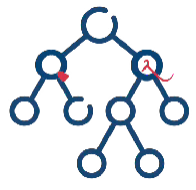
\includegraphics[height=0.9cm]{msca_logo.png}}%
  \end{center}
  \vspace{0.45cm}
  \begin{center}
    \begin{minipage}{0.1\textwidth}\centering
      \href{https://quantlet.com}{
\includegraphics[height=0.9cm]{ql_logo.png}}\end{minipage}%
    \begin{minipage}{0.78\textwidth}\centering
      {\Large\bfseries\usebeamercolor[fg]{title}\inserttitle}\par\vspace{0.25cm}
      {\large\usebeamercolor[fg]{title}\insertsubtitle}\end{minipage}%
    \begin{minipage}{0.1\textwidth}\centering
      \href{https://quantinar.com}{
\includegraphics[height=0.9cm]{qr_logo.png}}\end{minipage}
  \end{center}
  \vfill
  \hspace{0.4cm}{\bfseries\insertauthor}\par\vspace{0.12cm}
  \hspace{0.4cm}\begin{minipage}[t]{0.92\textwidth}\raggedright\footnotesize\insertinstitute\end{minipage}
  \par\vspace{0.4cm}}

% ---------------------------------------------------------------- lecture metadata
\newcommand{\nnshort}{}
\newcommand{\nnnb}{notebooks}
\newcommand{\nnrepo}{https://github.com/danpele/NEURAL_BIZ/tree/main}
% language-dependent labels (English default; \nnromanian switches to Romanian, call it before \nnlecture)
\newcommand{\txtcourse}{Neural Networks and Deep Learning}
\newcommand{\txtlecture}{Lecture}
\newcommand{\txtoutline}{Outline}
\newcommand{\txtintuition}{In one sentence:}
\newcommand{\txtjob}{In practice:}
\newcommand{\txttry}{Experiment yourself:}
\newcommand{\txtwhere}{where}
\newcommand{\txtsim}{SIMULATED DATA (teaching illustration)}
\newcommand{\txtnbsuffix}{}
\newcommand{\txtinstitute}{Bucharest University of Economic Studies (ASE), Department of Statistics and Econometrics\\
    Romanian Academy, Institute for Economic Forecasting (IPE)\\
    IDA Institute Digital Assets \textbullet\ AI4EFin \textbullet\ MSCA Digital Finance}
\newcommand{\nnromanian}{%
  \renewcommand{\txtcourse}{Rețele neuronale și deep learning}%
  \renewcommand{\txtlecture}{Cursul}%
  \renewcommand{\txtoutline}{Cuprins}%
  \renewcommand{\txtintuition}{Pe scurt:}%
  \renewcommand{\txtjob}{În practică:}%
  \renewcommand{\txttry}{Exercițiu practic:}%
  \renewcommand{\txtwhere}{unde}%
  \renewcommand{\txtsim}{DATE SIMULATE (doar pentru ilustrare)}%
  \renewcommand{\txtnbsuffix}{\string_ro}%
  \renewcommand{\txtinstitute}{Academia de Studii Economice din București (ASE), Departamentul de Statistică și Econometrie\\
    Academia Română, Institutul de Prognoză Economică (IPE)\\
    IDA Institute Digital Assets \textbullet\ AI4EFin \textbullet\ MSCA Digital Finance}}
\newcommand{\nnlecture}[2]{%
  \renewcommand{\nnshort}{\txtlecture\ #1}%
  \renewcommand{\nnnb}{notebooks/L#1\string_notebook\txtnbsuffix.ipynb}%
  \title[NN]{\txtcourse}%
  \subtitle{\txtlecture\ #1: #2}%
  \author{Prof.\ dr.\ Daniel Traian PELE}%
  \institute{\txtinstitute}%
  \date{}}

% ---------------------------------------------------------------- teaching blocks (one message per frame)
% \intuition{one plain sentence}  ->  formula with every symbol defined  ->  real-data example  ->  \manager{one line}
\newcommand{\intuition}[1]{\begin{itemize}\item {\color{MainBlue}\textbf{\txtintuition}}~#1\end{itemize}\vspace{0.6mm}}
\newcommand{\manager}[1]{\colorbox{Forest!10}{\parbox{\dimexpr\linewidth-2\fboxsep\relax}{\footnotesize
  \begin{itemize}\setlength{\itemsep}{0pt}\item \textbf{\color{Forest}\txtjob}~#1\end{itemize}}}}
% Experiment yourself: pointer to the matching notebook section
\newcommand{\tryit}[1]{{\scriptsize\href{\nnrepo/\nnnb}{%
  \raisebox{-0.15em}{
\includegraphics[height=0.85em]{ql_logo.png}}\,\textbf{\txttry}~\color{MainBlue}#1}}}
% bottom row: manager line (left) + experiment pointer (right), pinned to the bottom of the frame
\newcommand{\bottomrow}[2]{\par\vfill\noindent\begin{minipage}[b]{0.72\linewidth}#1\end{minipage}\hfill
  \begin{minipage}[b]{0.26\linewidth}\raggedleft #2\end{minipage}\par\vspace{0.5mm}}
\newcommand{\where}[1]{{\footnotesize\textbf{\txtwhere}~#1\par}}

% ---------------------------------------------------------------- helpers
% chart source line under a figure: \chartsource{Source ...; period ...}
\newcommand{\chartsource}[1]{\par\vspace{1pt}{\scriptsize\color{FooterGray}#1\par}}
% link to code: \quantlet{label}{path inside the repo}
\newcommand{\quantlet}[2]{\par\vspace{1pt}\hfill\href{\nnrepo/#2}{%
  \raisebox{-0.15em}{
\includegraphics[height=0.75em]{ql_logo.png}}\textcolor{MainBlue}{\scriptsize\ #1}}}
% inline Quantlet link for the bottom-right corner of a frame: \qlink{label}{path inside the repo}
\newcommand{\qlink}[2]{{\scriptsize\href{\nnrepo/#2}{\raisebox{-0.15em}{
\includegraphics[height=0.85em]{ql_logo.png}}\,\textcolor{MainBlue}{#1}}}}
\newcommand{\simlabel}{\colorbox{Crimson!12}{\scriptsize\bfseries\color{Crimson}\txtsim}}
\newcommand{\E}{\mathbb{E}}
\newcommand{\Var}{\operatorname{Var}}
\newcommand{\Cov}{\operatorname{Cov}}
\newcommand{\Corr}{\operatorname{Corr}}
\newcommand{\asinh}{\operatorname{asinh}}
\newcommand{\iid}{\overset{\text{i.i.d.}}{\sim}}
\newcommand{\EUR}{EUR}
% deep-learning notation (Bishop & Bishop, 2024): vectors bold lower case, matrices bold upper case
\newcommand{\R}{\mathbb{R}}
\newcommand{\vx}{\mathbf{x}}
\newcommand{\vy}{\mathbf{y}}
\newcommand{\vz}{\mathbf{z}}
\newcommand{\vh}{\mathbf{h}}
\newcommand{\vw}{\mathbf{w}}
\newcommand{\vb}{\mathbf{b}}
\newcommand{\mW}{\mathbf{W}}
\newcommand{\mX}{\mathbf{X}}
\newcommand{\btheta}{\boldsymbol{\theta}}
\newcommand{\loss}{\mathcal{L}}
\newcommand{\dataset}{\mathcal{D}}
\DeclareMathOperator*{\argmin}{arg\,min}
\DeclareMathOperator*{\argmax}{arg\,max}
\DeclareMathOperator{\softmax}{softmax}
\DeclareMathOperator{\ReLU}{ReLU}
\DeclareMathOperator{\sigm}{\sigma}

\nnlecture{4}{Convolutional neural networks (CNN) and transfer learning}
\begin{document}
{\setbeamertemplate{headline}{}\setbeamertemplate{footline}{}
\begin{frame}\titlepage\end{frame}}
% END-FRONT-MATTER

\begin{frame}{Learning objectives}
\small
\begin{itemize}\setlength{\itemsep}{4pt}
  \item Write a convolutional layer as a formula: kernel, padding, stride, channels, parameters and receptive field.
  \item Explain why a convolutional neural network (CNN) needs far fewer parameters than a multilayer perceptron (MLP) on images, and verify it on real data.
  \item Read the classic architectures, from LeNet to ResNet, and the residual connection that makes deep networks trainable.
  \item Use transfer learning (feature extraction and fine-tuning) when labelled images are expensive, and measure what it saves.
  \item Explain a prediction with a gradient-weighted class activation map (CAM) and turn image predictions into business numbers.
\end{itemize}
\end{frame}

% BEGIN-ABBR

\begin{frame}{Abbreviations}
\small
\vspace{-1mm}\begin{columns}[T,onlytextwidth]
\begin{column}{0.49\textwidth}{\scriptsize\renewcommand{\arraystretch}{0.96}\begin{tabular}{@{}>{\bfseries}l@{\ \ }p{0.74\linewidth}@{}}AI & artificial intelligence\\
ASE & Bucharest University of Economic Studies\\
BN & batch normalisation\\
CAM & class activation map\\
CIFAR & Canadian Institute for Advanced Research (CIFAR-10 image set)\\
CNN & convolutional neural network\\
CPU & central processing unit\\
EU & European Union\\
GAP & global average pooling\\
GPT & generative pre-trained transformer\\
GPU & graphics processing unit\\\end{tabular}}\end{column}
\begin{column}{0.49\textwidth}{\scriptsize\renewcommand{\arraystretch}{0.96}\begin{tabular}{@{}>{\bfseries}l@{\ \ }p{0.74\linewidth}@{}}ICBE & International Conference on Business Excellence\\
IPE & Institute for Economic Forecasting, Romanian Academy\\
MLP & multilayer perceptron\\
MNIST & Modified National Institute of Standards and Technology (digit images)\\
MPS & Metal Performance Shaders (Apple GPU back end of PyTorch)\\
ReLU & rectified linear unit\\
RGB & red, green, blue (colour channels)\\
SGD & stochastic gradient descent\\
VGG & Visual Geometry Group, University of Oxford\\
VLM & vision--language model\\\end{tabular}}\end{column}
\end{columns}
\end{frame}

% END-ABBR

\begin{frame}{Real data only: three image collections}
\footnotesize

\par\vspace{0.5mm}{\scriptsize \begin{itemize}\setlength{\itemsep}{0pt}
  \item The Modified National Institute of Standards and Technology (MNIST) digits are replaced in Fashion-MNIST by clothing photos; the Canadian Institute for Advanced Research (CIFAR) released CIFAR-10.
\end{itemize}}{\footnotesize\renewcommand{\arraystretch}{1.05}\setlength{\tabcolsep}{4pt}
\begin{tabular}{@{}p{0.2\textwidth}p{0.3\textwidth}p{0.2\textwidth}p{0.22\textwidth}@{}}\toprule
Data set & Content & Split (train/valid/test) & Business use \\ \midrule
Fashion-MNIST & Zalando catalogue photos, 10 product types, 28$\times$28 grey & 50\,000 / 10\,000 / 10\,000 & automatic product tagging \\
CIFAR-10 & photographs, 10 object classes, 32$\times$32 colour & 45\,000 / 5\,000 / 10\,000 & benchmark for architectures \\
EuroSAT & Sentinel-2 satellite tiles of Europe, 10 land-use classes, 64$\times$64 colour & 16\,200 / 5\,400 / 5\,400 & agriculture, insurance, real estate \\
\bottomrule\end{tabular}}
\par\vspace{0.5mm}{\scriptsize \begin{itemize}\setlength{\itemsep}{0pt}
  \item Sources: Zalando Research (Xiao et al., 2017); Krizhevsky (2009); Helber et al. (2019), Copernicus Sentinel-2 data; all downloaded by the course scripts (data/SOURCES.md).
  \item Validation parts are used for early stopping and tuning; every test set is used once, at the end.
  \item Pre-trained weights: ResNet-18 trained on ImageNet (torchvision); training on an Apple graphics processing unit (GPU) through Metal Performance Shaders (MPS), seed 20261108.
\end{itemize}}
\par\vfill\noindent{\scriptsize\color{FooterGray}(data/SOURCES.md)}\par\vspace{0.5mm}
\end{frame}


\section{Images as data: why convolutions}

\begin{frame}{A product photo is a matrix of numbers}
\small
\intuition{each image is a $28\times28$ array of grey levels; a model must map it to one of 10 product types.}
\vspace{-1mm}\[ \mathbf{X}\in[0,1]^{28\times 28},\qquad \hat{\mathbf p}=f_{\btheta}(\mathbf X)\in\Delta^{9},\qquad \hat y=\argmax_k \hat p_k \]\vspace{-2mm}
\begin{center}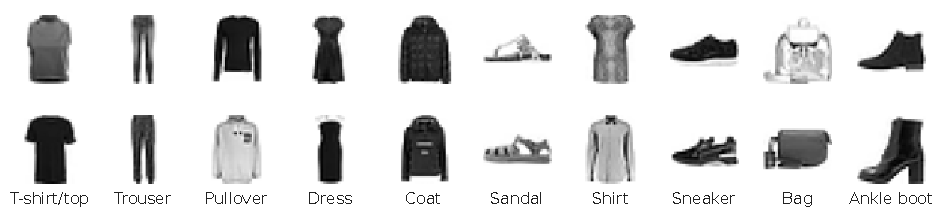
\includegraphics[width=\textwidth,height=0.327\textheight,keepaspectratio]{charts/en/fmnist_samples.pdf}\end{center}\vspace{-3mm}
\chartsource{Source: Fashion-MNIST, Zalando Research (Xiao et al., 2017). Data: 60,000 training images, 28 x 28 grey levels.}
\vspace{0.5mm}
\begin{itemize}\setlength{\itemsep}{0pt}
  \item Fashion-MNIST: 50\,000 training, 10\,000 validation and 10\,000 test images from the Zalando catalogue.
\end{itemize}
\par\vfill\manager{an online retailer tags thousands of new product photos a day
    \begin{itemize}\setlength{\itemsep}{0pt}
      \item A classifier sets the category, a person checks the doubtful ones.
    \end{itemize}}\par\vspace{0.5mm}
\par\vfill\noindent{\scriptsize\color{FooterGray}(Xiao et al., 2017)}\hfill\qlink{NN\_L4\_fmnist\_samples}{Quantlets/L4/NN_L4_fmnist_samples}\par\vspace{0.5mm}
\end{frame}

\begin{frame}{A dense layer on pixels wastes parameters and ignores space}
\footnotesize
\intuition{an MLP treats pixel (1,1) and pixel (1,2) as unrelated inputs and needs one weight per pixel and unit.}
\begin{columns}[T,onlytextwidth]
\begin{column}{0.53\textwidth}
\[ \mathbf h=\sigma(\mW\,\mathrm{vec}(\mathbf X)+\vb),\quad \mW\in\R^{m\times HWC} \]{\footnotesize\begin{itemize}\setlength{\itemsep}{0pt}
  \item \textbf{\txtwhere}
    \begin{itemize}\setlength{\itemsep}{0pt}
      \item $H,W$ height and width
      \item $C$ channels
      \item $m$ hidden units
      \item A $224\times224$ colour image and $m=1000$ give $224\cdot224\cdot3\cdot1000\approx1.5\cdot10^{8}$ weights in the first layer alone
    \end{itemize}
\end{itemize}\par}
\end{column}
\begin{column}{0.44\textwidth}
\begin{itemize}\setlength{\itemsep}{2pt}
  \item \textbf{Three ideas of a CNN}
    \begin{itemize}\setlength{\itemsep}{0pt}
      \item Local connectivity: a unit sees a small patch
      \item Weight sharing: the same filter at every position
      \item Equivariance: shifting the input shifts the feature map, $f(T_{\delta}\mathbf X)=T_{\delta}f(\mathbf X)$
    \end{itemize}
  \item On our data: MLP 235\,146 parameters, CNN 140\,778, 1.67 times fewer.
\end{itemize}
\end{column}
\end{columns}
\par\vfill\manager{fewer parameters mean less data needed for the same accuracy, which is what labelled business images cost.}\par\vspace{0.5mm}
\par\vfill\noindent{\scriptsize\color{FooterGray}(LeCun et al., 1998; Bishop \& Bishop, 2024, ch.~10)}\par\vspace{0.5mm}
\end{frame}


\section{The convolutional layer, formula by formula}

\begin{frame}{Convolution: the same small filter slides over the image}
\footnotesize
\intuition{each output value is a weighted sum of a $k\times k$ neighbourhood, with weights shared across positions.}
\begin{columns}[T,onlytextwidth]
\begin{column}{0.64\textwidth}
\[ Z_{o}(i,j)=b_o+\sum_{c=1}^{C_{\mathrm{in}}}\sum_{u=0}^{k-1}\sum_{v=0}^{k-1}K_{o,c}(u,v)\,X_c(i s+u-p,\;j s+v-p) \]{\footnotesize\begin{itemize}\setlength{\itemsep}{0pt}
  \item \textbf{\txtwhere}
    \begin{itemize}\setlength{\itemsep}{0pt}
      \item $X_c$ input channel $c$
      \item $K_{o,c}$ the $k\times k$ kernel from channel $c$ to output map $o$
      \item $b_o$ bias
      \item $s$ stride
      \item $p$ zero padding
    \end{itemize}
\end{itemize}\par}
\end{column}
\begin{column}{0.33\textwidth}
\begin{itemize}\setlength{\itemsep}{2pt}
  \item Feature map of filter $o$: $A_o=\ReLU(Z_o)$, with the rectified linear unit (ReLU) $\max(0,z)$
    \begin{itemize}\setlength{\itemsep}{0pt}
      \item $K$ is learned by backpropagation.
    \end{itemize}
\end{itemize}
\end{column}
\end{columns}
\par\vfill\manager{a filter is a pattern detector that is tested at every position of the image at the cost of $k^2C_{\mathrm{in}}$ weights.}\par\vspace{0.5mm}
\par\vfill\noindent{\scriptsize\color{FooterGray}(Goodfellow et al., 2016, ch.~9)}\par\vspace{0.5mm}
\end{frame}

\begin{frame}{Hand-made filters already find roads and field edges}
\small
\intuition{a Sobel kernel responds where the brightness changes along one direction; a mean kernel blurs.}
\vspace{-1mm}\[ K_x=\begin{psmallmatrix}-1&0&1\\-2&0&2\\-1&0&1\end{psmallmatrix},\quad K_y=K_x^{\top},\quad K_{\mathrm{mean}}=\tfrac19\mathbf 1_{3\times3} \]\vspace{-2mm}
\begin{center}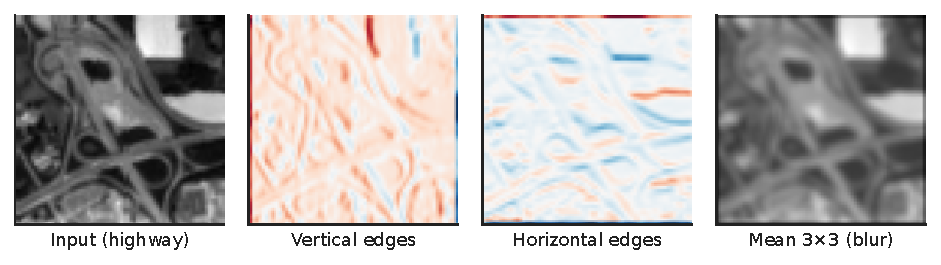
\includegraphics[width=\textwidth,height=0.360\textheight,keepaspectratio]{charts/en/conv_edges.pdf}\end{center}\vspace{-3mm}
\chartsource{Source: EuroSAT, Sentinel-2 images (Helber et al., 2019). Data: one 64 x 64 Sentinel-2 tile (class Highway), grey levels.}
\vspace{0.5mm}
\begin{itemize}\setlength{\itemsep}{0pt}
  \item Padding $p=1$ keeps the $64\times64$ size
    \begin{itemize}\setlength{\itemsep}{0pt}
      \item A CNN learns dozens of such kernels per layer instead of fixing them.
    \end{itemize}
\end{itemize}
\par\vfill\noindent{\scriptsize\color{FooterGray}(own computation)}\hfill\qlink{NN\_L4\_conv\_edges}{Quantlets/L4/NN_L4_conv_edges}\par\vspace{0.5mm}
\end{frame}

\begin{frame}{Output size, padding and stride}
\footnotesize
\intuition{three integers decide how large each feature map is.}
\begin{columns}[T,onlytextwidth]
\begin{column}{0.53\textwidth}
\[ H_{\mathrm{out}}=\Big\lfloor\frac{H_{\mathrm{in}}+2p-k}{s}\Big\rfloor+1 \]{\footnotesize\begin{itemize}\setlength{\itemsep}{0pt}
  \item \textbf{\txtwhere}
    \begin{itemize}\setlength{\itemsep}{0pt}
      \item $H_{\mathrm{in}}$ input height (same formula for width)
      \item $k$ kernel size
      \item $p$ padding
      \item $s$ stride
    \end{itemize}
\end{itemize}\par}
\end{column}
\begin{column}{0.44\textwidth}
\begin{itemize}\setlength{\itemsep}{2pt}
  \item \textbf{Worked examples}, $H_{\mathrm{in}}=64$, $k=3$
    \begin{itemize}\setlength{\itemsep}{0pt}
      \item $p=1,s=1$: $H_{\mathrm{out}}=64$ (``same'')
      \item $p=0,s=1$: $H_{\mathrm{out}}=62$ (``valid'')
      \item $p=1,s=2$: $H_{\mathrm{out}}=32$ (downsampling)
    \end{itemize}
  \item Parameters of the layer: $(k^2C_{\mathrm{in}}+1)\,C_{\mathrm{out}}$, independent of the image size.
\end{itemize}
\end{column}
\end{columns}
\par\vfill\manager{the same network runs on any image size
    \begin{itemize}\setlength{\itemsep}{0pt}
      \item Only the cost in operations, $H_{\mathrm{out}}W_{\mathrm{out}}k^2C_{\mathrm{in}}C_{\mathrm{out}}$, grows.
    \end{itemize}}\par\vspace{0.5mm}
\par\vfill\noindent{\scriptsize\color{FooterGray}(own computation)}\par\vspace{0.5mm}
\end{frame}

\begin{frame}{Pooling summarises a neighbourhood; global pooling summarises the image}
\footnotesize
\intuition{max pooling keeps the strongest response in each window and makes the map smaller and slightly shift-invariant.}
\begin{columns}[T,onlytextwidth]
\begin{column}{0.53\textwidth}
\[ P_o(i,j)=\max_{0\le u,v<2}A_o(2i+u,2j+v) \]\vspace{-2mm}\[ g_o=\frac{1}{HW}\sum_{i,j}A_o(i,j) \]{\footnotesize\begin{itemize}\setlength{\itemsep}{0pt}
  \item \textbf{\txtwhere}
    \begin{itemize}\setlength{\itemsep}{0pt}
      \item $P_o$ max pooling $2\times2$, stride 2 (halves height and width)
      \item $g_o$ global average pooling (GAP), one number per channel
    \end{itemize}
\end{itemize}\par}
\end{column}
\begin{column}{0.44\textwidth}
\begin{itemize}\setlength{\itemsep}{2pt}
  \item Our Fashion-MNIST CNN: maps $28\times28\to14\times14\to7\times7$, then GAP gives 128 numbers and one linear layer gives the 10 class scores.
  \item Gradient of max pooling: it flows only to the arg-max position of each window.
  \item GAP replaces large dense layers (thousands of weights) by an average (zero weights).
\end{itemize}
\end{column}
\end{columns}
\par\vfill\manager{GAP is the reason a modern CNN has few parameters in its head and can be explained with class activation maps.}\par\vspace{0.5mm}
\par\vfill\noindent{\scriptsize\color{FooterGray}(Bishop \& Bishop, 2024, sec.~10.2)}\par\vspace{0.5mm}
\end{frame}

\begin{frame}{Depth, pooling and the receptive field}
\small
\intuition{the receptive field is the patch of the input that can influence one unit.}
\vspace{-1mm}\[ r_l=r_{l-1}+(k_l-1)\prod_{i<l}s_i,\qquad r_0=1 \]\vspace{-2mm}
\begin{center}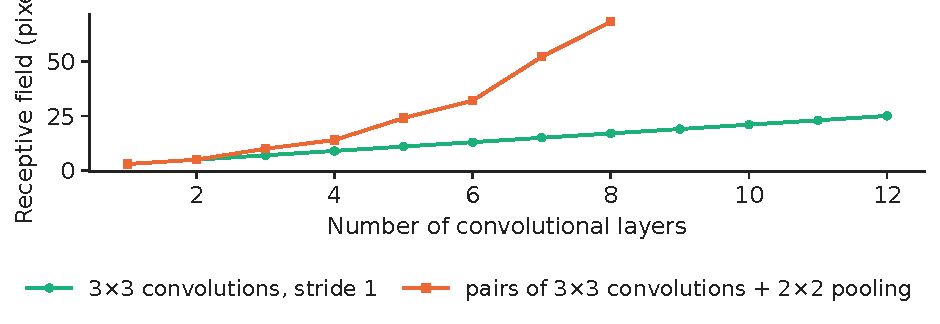
\includegraphics[width=\textwidth,height=0.360\textheight,keepaspectratio]{charts/en/receptive_field.pdf}\end{center}\vspace{-3mm}
\chartsource{Source: own computation from the receptive-field recursion. Data: recursion of the receptive field, no data.}
\vspace{0.5mm}
\begin{itemize}\setlength{\itemsep}{0pt}
  \item Twelve $3\times3$ layers at stride 1 see only $25\times25$ pixels
    \begin{itemize}\setlength{\itemsep}{0pt}
      \item Eight with $2\times2$ pooling after every pair see $68\times68$.
    \end{itemize}
\end{itemize}
\par\vfill\noindent{\scriptsize\color{FooterGray}(own computation)}\hfill\qlink{NN\_L4\_receptive\_field}{Quantlets/L4/NN_L4_receptive_field}\par\vspace{0.5mm}
\end{frame}

\begin{frame}{Backpropagation through a convolution is again a convolution}
\footnotesize
\intuition{because the kernel is shared, its gradient sums the contributions of every position.}
\begin{columns}[T,onlytextwidth]
\begin{column}{0.53\textwidth}
\[ \frac{\partial\loss}{\partial K_{o,c}(u,v)}=\sum_{i,j}\delta_o(i,j)\,X_c(is+u-p,\,js+v-p) \]\vspace{-2mm}\[ \delta_o(i,j)=\frac{\partial\loss}{\partial Z_o(i,j)} \]{\footnotesize\begin{itemize}\setlength{\itemsep}{0pt}
  \item \textbf{\txtwhere}
    \begin{itemize}\setlength{\itemsep}{0pt}
      \item $\delta_o$ the error map of output $o$, computed by backpropagation from the layer above
      \item For $s=1$, $\partial\loss/\partial X_c=\sum_o \delta_o \star \mathrm{rot}_{180}(K_{o,c})$, a full convolution
    \end{itemize}
\end{itemize}\par}
\end{column}
\begin{column}{0.44\textwidth}
\begin{itemize}\setlength{\itemsep}{2pt}
  \item Weight sharing turns millions of position-specific gradients into one sum per weight.
  \item In code, autograd does it: \texttt{loss.backward()} on a \texttt{nn.Conv2d}.
  \item Derivation in the appendix (convolution as a matrix product).
\end{itemize}
\end{column}
\end{columns}
\par\vfill\manager{one forward and one backward pass cost about the same number of operations, so training time scales with the forward cost.}\par\vspace{0.5mm}
\par\vfill\noindent{\scriptsize\color{FooterGray}(Goodfellow et al., 2016, sec.~9.5)}\par\vspace{0.5mm}
\end{frame}

\begin{frame}{Batch normalisation keeps every channel on the same scale}
\footnotesize
\intuition{each channel is standardised over the batch and the positions, then rescaled by two learned numbers.}
\begin{columns}[T,onlytextwidth]
\begin{column}{0.53\textwidth}
\[ \hat a=\frac{a-\mu_{\mathcal B,o}}{\sqrt{\sigma^2_{\mathcal B,o}+\epsilon}},\qquad \mathrm{BN}(a)=\gamma_o\hat a+\beta_o \]{\footnotesize\begin{itemize}\setlength{\itemsep}{0pt}
  \item \textbf{\txtwhere}
    \begin{itemize}\setlength{\itemsep}{0pt}
      \item $\mu_{\mathcal B,o},\sigma^2_{\mathcal B,o}$ mean and variance of channel $o$ over the batch $\mathcal B$ and all positions
      \item $\gamma_o,\beta_o$ learned
      \item At test time running averages replace the batch statistics
    \end{itemize}
\end{itemize}\par}
\end{column}
\begin{column}{0.44\textwidth}
\begin{itemize}\setlength{\itemsep}{2pt}
  \item Every network of this lecture uses batch normalisation (BN) after each convolution: Conv $\to$ BN $\to$ ReLU.
  \item It allows larger learning rates
    \begin{itemize}\setlength{\itemsep}{0pt}
      \item Our CIFAR runs use a one-cycle schedule up to 0.1 (chosen a priori).
    \end{itemize}
  \item Remember \texttt{model.eval()} before prediction: otherwise BN uses the test batch.
\end{itemize}
\end{column}
\end{columns}
\par\vfill\manager{a model that scores well in the notebook but badly in production often forgot eval mode or the input scaling of training.}\par\vspace{0.5mm}
\par\vfill\noindent{\scriptsize\color{FooterGray}(Ioffe \& Szegedy, 2015)}\par\vspace{0.5mm}
\end{frame}


\section{Case study: product photos, from softmax to CNN}

\begin{frame}{Experimental protocol for the three models}
\footnotesize
\begin{columns}[T,onlytextwidth]
\begin{column}{0.5\textwidth}
\begin{itemize}\setlength{\itemsep}{3pt}
  \item \textbf{Benchmark}: softmax (multinomial logistic) regression
    \begin{itemize}\setlength{\itemsep}{0pt}
      \item $\hat{\mathbf p}=\softmax(\mW\mathrm{vec}(\mathbf X)+\vb)$, 7\,850 parameters
    \end{itemize}
  \item \textbf{MLP}: 784--256--128--10, ReLU, dropout 0.2
    \begin{itemize}\setlength{\itemsep}{0pt}
      \item 235\,146 parameters
    \end{itemize}
  \item \textbf{CNN}: 2 blocks [Conv3$\times$3--BN--ReLU]$\times$2 + max pool, Conv 128, GAP, linear
    \begin{itemize}\setlength{\itemsep}{0pt}
      \item 140\,778 parameters
    \end{itemize}
\end{itemize}
\end{column}
\begin{column}{0.47\textwidth}
\begin{itemize}\setlength{\itemsep}{3pt}
  \item \textbf{Same training for all}
    \begin{itemize}\setlength{\itemsep}{0pt}
      \item AdamW, batch 128, 12 epochs, one-cycle learning rate
      \item Cross-entropy $\loss=-\frac1n\sum_i\log\hat p_{i,y_i}$
      \item Pixels standardised with the training mean 0.2859 and standard deviation 0.3530
    \end{itemize}
  \item \textbf{Fair comparison}
    \begin{itemize}\setlength{\itemsep}{0pt}
      \item Early stopping on the 10\,000 validation images
      \item 3 seeds per model; test images used once
    \end{itemize}
\end{itemize}
\end{column}
\end{columns}
\par\vfill\manager{total training time of the nine runs: 299 seconds on the GPU of a laptop.}\par\vspace{0.5mm}
\par\vfill\noindent{\scriptsize\color{FooterGray}(own computation)}\hfill\tryit{\S3}\par\vspace{0.5mm}
\end{frame}

\begin{frame}{The CNN learns faster and generalises better}
\small
\intuition{validation loss falls lowest for the CNN; the MLP fits the training data but stops improving on new images.}
\begin{center}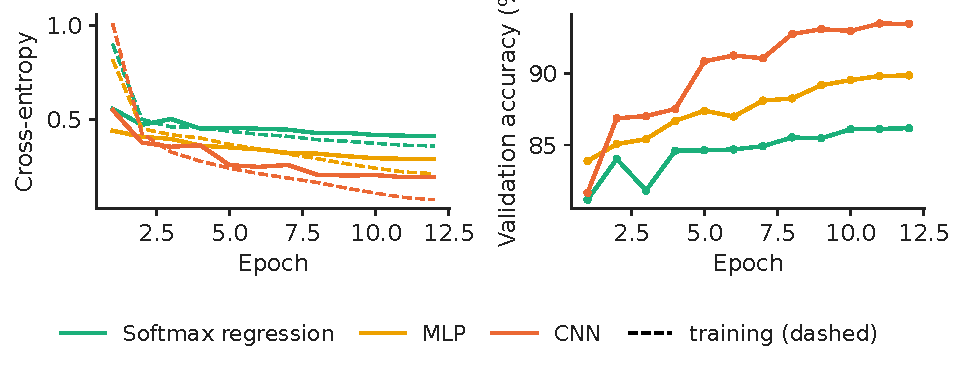
\includegraphics[width=\textwidth,height=0.500\textheight,keepaspectratio]{charts/en/fmnist_curves.pdf}\end{center}\vspace{-3mm}
\chartsource{Source: Fashion-MNIST, Zalando Research (Xiao et al., 2017). Data: 50,000 training and 10,000 validation images; seed 20261108.}
\vspace{0.5mm}
\begin{itemize}\setlength{\itemsep}{0pt}
  \item Best validation epoch (seed 20261108): CNN 11, MLP 12, softmax 12, out of 12.
\end{itemize}
\par\vfill\noindent{\scriptsize\color{FooterGray}(own computation)}\hfill\qlink{NN\_L4\_fmnist\_curves}{Quantlets/L4/NN_L4_fmnist_curves}\par\vspace{0.5mm}
\end{frame}

\begin{frame}{Higher accuracy with fewer parameters}
\small
\intuition{weight sharing buys accuracy and saves parameters at the same time.}
\begin{center}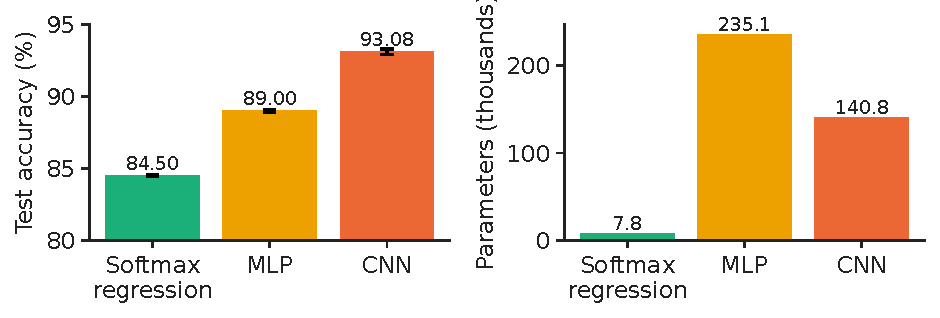
\includegraphics[width=\textwidth,height=0.420\textheight,keepaspectratio]{charts/en/fmnist_compare.pdf}\end{center}\vspace{-3mm}
\chartsource{Source: Fashion-MNIST, Zalando Research (Xiao et al., 2017). Data: 10,000 test images; mean and standard deviation over 3 seeds.}
\vspace{0.5mm}
\begin{itemize}\setlength{\itemsep}{0pt}
  \item Test accuracy (mean $\pm$ sd, 3 seeds): softmax 84.50\,$\pm$\,0.06\,\%, MLP 89.00\,$\pm$\,0.10\,\%, CNN 93.08\,$\pm$\,0.20\,\%.
  \item The CNN removes 37.1\,\% of the MLP's errors with 1.67 times fewer parameters.
\end{itemize}
\par\vfill\noindent{\scriptsize\color{FooterGray}(own computation)}\hfill\qlink{NN\_L4\_fmnist\_compare}{Quantlets/L4/NN_L4_fmnist_compare}\par\vspace{0.5mm}
\end{frame}

\begin{frame}{McNemar's test of the accuracy gain on the same test images}
\footnotesize
\intuition{two classifiers scored on the same images differ only through the images on which exactly one of them is right.}
\begin{columns}[T,onlytextwidth]
\begin{column}{0.53\textwidth}
\[ \chi^2=\frac{(|b-c|-1)^2}{b+c}\;\overset{H_0}{\sim}\;\chi^2_1 \]{\footnotesize\begin{itemize}\setlength{\itemsep}{0pt}
  \item \textbf{\txtwhere}
    \begin{itemize}\setlength{\itemsep}{0pt}
      \item $b$ images right for the CNN only
      \item $c$ right for the MLP only
      \item $H_0$: both have the same error rate
      \item 5\,\% critical value 3.84
    \end{itemize}
\end{itemize}\par}
\end{column}
\begin{column}{0.44\textwidth}
\begin{itemize}\setlength{\itemsep}{2pt}
  \item Seed 20261108: $b=614$, $c=226$, $\chi^2=178.3$: the null is rejected.
  \item Across the 3 seeds, the paired $t$ statistic of the accuracy gap is 31.38.
  \item Seeds measure the training noise
    \begin{itemize}\setlength{\itemsep}{0pt}
      \item McNemar measures the test-set noise
      \item Report both.
    \end{itemize}
\end{itemize}
\end{column}
\end{columns}
\par\vfill\manager{before replacing a production model, show that the gain survives a test on the same cases, not only a higher average.}\par\vspace{0.5mm}
\par\vfill\noindent{\scriptsize\color{FooterGray}(McNemar, 1947)}\par\vspace{0.5mm}
\end{frame}

\begin{frame}{The errors are the products that people also confuse}
\small
\intuition{most mistakes are between upper-body garments of similar shape.}
\begin{center}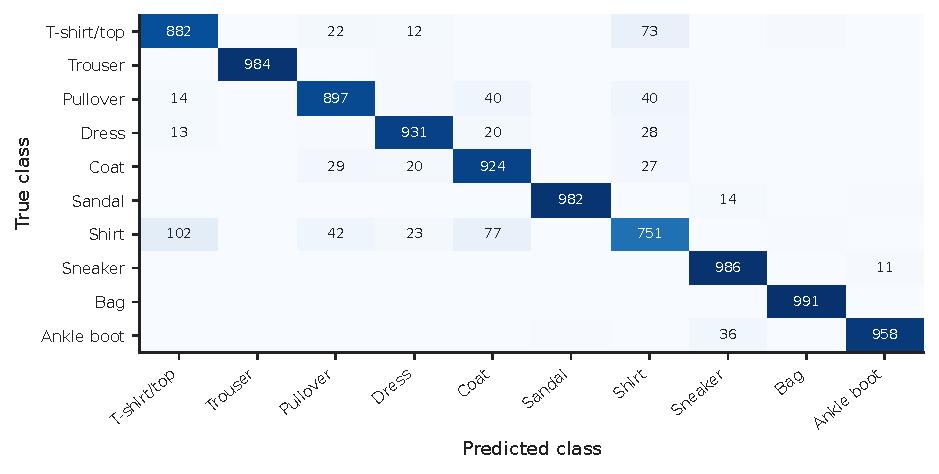
\includegraphics[width=\textwidth,height=0.432\textheight,keepaspectratio]{charts/en/fmnist_confusion.pdf}\end{center}\vspace{-3mm}
\chartsource{Source: Fashion-MNIST, Zalando Research (Xiao et al., 2017). Data: 10,000 test images, CNN seed 20261108.}
\vspace{0.5mm}
\begin{itemize}\setlength{\itemsep}{0pt}
  \item Weakest class: Shirt (recall 75.1\,\%)
    \begin{itemize}\setlength{\itemsep}{0pt}
      \item Largest confusion: Shirt taken for T-shirt/top, 102 images.
    \end{itemize}
\end{itemize}
\par\vfill\manager{route only low-confidence photos of the weak classes to a human: the error cost falls where it is highest.}\par\vspace{0.5mm}
\par\vfill\noindent{\scriptsize\color{FooterGray}(own computation)}\hfill\qlink{NN\_L4\_fmnist\_confusion}{Quantlets/L4/NN_L4_fmnist_confusion}\par\vspace{0.5mm}
\end{frame}

\begin{frame}{First-layer filters are edge and contrast detectors}
\small
\intuition{nobody told the network to look for edges; gradient descent found them.}
\begin{center}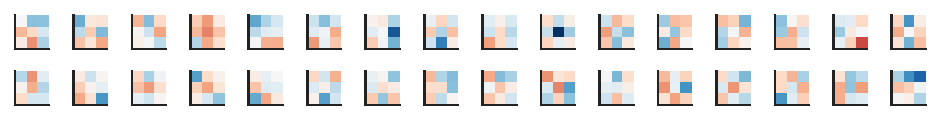
\includegraphics[width=\textwidth,height=0.200\textheight,keepaspectratio]{charts/en/fmnist_filters.pdf}\end{center}\vspace{-3mm}
\chartsource{Source: Fashion-MNIST, Zalando Research (Xiao et al., 2017). Data: first convolutional layer of the CNN (32 filters of 3 x 3), seed 20261108.}
\vspace{0.5mm}
\begin{itemize}\setlength{\itemsep}{0pt}
  \item Red = positive weight, blue = negative: many kernels are oriented differences, like the Sobel kernels set by hand.
  \item Deeper layers combine them into parts (collars, soles, handles) (Zeiler \& Fergus, 2014).
\end{itemize}
\par\vfill\noindent{\scriptsize\color{FooterGray}(own computation; Zeiler \& Fergus, 2014)}\hfill\qlink{NN\_L4\_fmnist\_filters}{Quantlets/L4/NN_L4_fmnist_filters}\par\vspace{0.5mm}
\end{frame}

\begin{frame}{Feature maps: from edges to a coarse map of parts}
\small
\intuition{early maps keep the outline of the boot; deep maps are small but say where the informative parts are.}
\begin{center}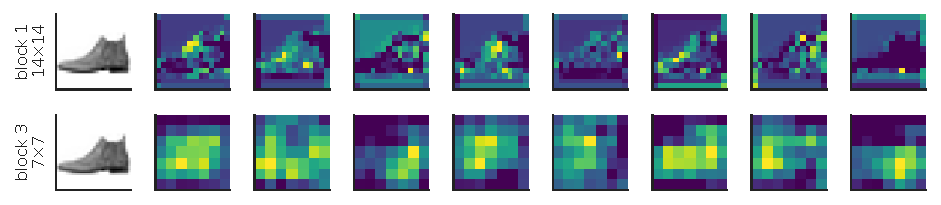
\includegraphics[width=\textwidth,height=0.360\textheight,keepaspectratio]{charts/en/fmnist_featuremaps.pdf}\end{center}\vspace{-3mm}
\chartsource{Source: Fashion-MNIST, Zalando Research (Xiao et al., 2017). Data: one test image (ankle boot); 8 most active channels per block.}
\vspace{0.5mm}
\begin{itemize}\setlength{\itemsep}{0pt}
  \item Block 1: 32 maps of 14$\times$14
    \begin{itemize}\setlength{\itemsep}{0pt}
      \item Block 3: 128 maps of 7$\times$7, then averaged by GAP.
    \end{itemize}
\end{itemize}
\par\vfill\noindent{\scriptsize\color{FooterGray}(own computation)}\hfill\qlink{NN\_L4\_fmnist\_featuremaps}{Quantlets/L4/NN_L4_fmnist_featuremaps}\par\vspace{0.5mm}
\end{frame}


\section{Architectures: from LeNet to ResNet}

\begin{frame}{Image-recognition architectures, 1998--2021}
\footnotesize
{\footnotesize\renewcommand{\arraystretch}{1.05}\setlength{\tabcolsep}{4pt}
\begin{tabular}{@{}p{0.17\textwidth}p{0.07\textwidth}p{0.68\textwidth}@{}}\toprule
Network & Year & Key idea \\ \midrule
LeNet-5 & 1998 & convolution + subsampling for handwritten digits (the MNIST benchmark); trained by backpropagation \\
AlexNet & 2012 & deep CNN on ImageNet trained on GPUs; ReLU, dropout, data augmentation \\
Visual Geometry Group (VGG) & 2015 & only $3\times3$ kernels: two stacked $3\times3$ see $5\times5$ with $18C^2$ instead of $25C^2$ weights \\
ResNet & 2016 & residual connections $\mathbf y=\mathbf x+F(\mathbf x)$: networks of 100+ layers become trainable \\
Vision transformer & 2021 & image patches as tokens with attention (Lecture 7) \\
\bottomrule\end{tabular}}
\par\vspace{0.5mm}{\scriptsize \begin{itemize}\setlength{\itemsep}{0pt}
  \item ResNet-18, used for transfer learning below, has 11\,181\,642 parameters (our count, with a 10-class head).
\end{itemize}}
\par\vfill\noindent{\scriptsize\color{FooterGray}(LeCun et al., 1998; Krizhevsky et al., 2012; Simonyan \& Zisserman, 2015; He et al., 2016)}\par\vspace{0.5mm}
\end{frame}

\begin{frame}{Residual connections and the identity path}
\footnotesize
\intuition{a block adds its output to its input, so the gradient always has a direct path back.}
\begin{columns}[T,onlytextwidth]
\begin{column}{0.53\textwidth}
\[ \mathbf y=\ReLU\big(\mathbf x+F(\mathbf x;\mW)\big),\qquad \frac{\partial\loss}{\partial\mathbf x}=\frac{\partial\loss}{\partial\mathbf y}\Big(\mathbf I+\frac{\partial F}{\partial\mathbf x}\Big) \]{\footnotesize\begin{itemize}\setlength{\itemsep}{0pt}
  \item \textbf{\txtwhere}
    \begin{itemize}\setlength{\itemsep}{0pt}
      \item $F$ two Conv--BN layers
      \item When the shape changes, $\mathbf x$ passes through a $1\times1$ convolution with stride 2
      \item The derivative is written for the pre-activation sum
    \end{itemize}
\end{itemize}\par}
\end{column}
\begin{column}{0.44\textwidth}
\begin{itemize}\setlength{\itemsep}{2pt}
  \item Plain deep networks suffer from degradation: deeper ones have higher training error, which is an optimisation problem, not overfitting.
  \item If the best block is the identity, it suffices to set $F=0$.
  \item On CIFAR-10 (next frame): same 32 layers, with and without the shortcut.
\end{itemize}
\end{column}
\end{columns}
\par\vfill\manager{residual blocks are the default in every modern vision and language model, including transformers.}\par\vspace{0.5mm}
\par\vfill\noindent{\scriptsize\color{FooterGray}(He et al., 2016)}\par\vspace{0.5mm}
\end{frame}

\begin{frame}{Augmentation narrows the gap; residuals make depth trainable}
\small
\intuition{left: the same CNN on Canadian Institute for Advanced Research (CIFAR-10) photos; right: 32-layer networks that differ only by the shortcut.}
\begin{center}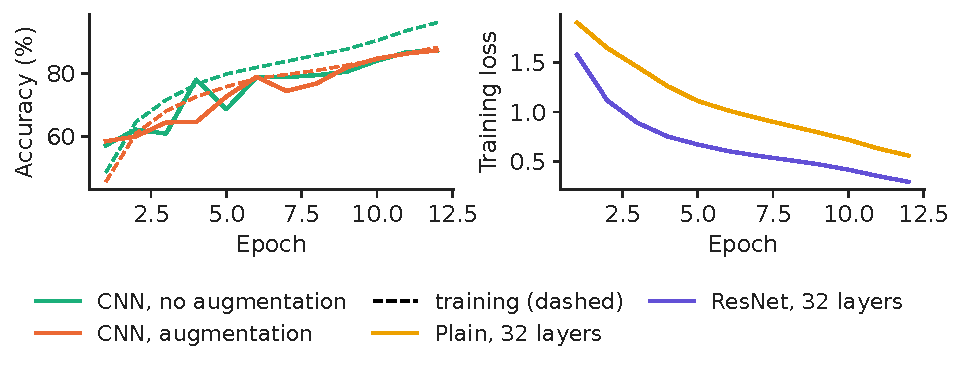
\includegraphics[width=\textwidth,height=0.420\textheight,keepaspectratio]{charts/en/cifar_curves.pdf}\end{center}\vspace{-3mm}
\chartsource{Source: CIFAR-10 (Krizhevsky, 2009). Data: 45,000 training and 5,000 validation images; seed 20261108.}
\vspace{0.5mm}
\begin{itemize}\setlength{\itemsep}{0pt}
  \item Test accuracy: CNN 86.56\,\% without and 86.86\,\% with augmentation (train--valid gap 8.9 vs 0.9 points).
  \item Plain-32 79.96\,\% vs ResNet-32 87.81\,\%
    \begin{itemize}\setlength{\itemsep}{0pt}
      \item Final training loss 0.557 vs 0.291.
    \end{itemize}
\end{itemize}
\par\vfill\noindent{\scriptsize\color{FooterGray}(own computation)}\hfill\qlink{NN\_L4\_cifar\_curves}{Quantlets/L4/NN_L4_cifar_curves}\par\vspace{0.5mm}
\end{frame}

\begin{frame}{Data augmentation as prior information}
\footnotesize
\intuition{we train on random transformations that should not change the label, which averages the loss over them.}
\begin{columns}[T,onlytextwidth]
\begin{column}{0.53\textwidth}
\[ \min_{\btheta}\;\frac1n\sum_{i=1}^n\E_{T\sim\mathcal T}\Big[\ell\big(f_{\btheta}(T(\mathbf X_i)),y_i\big)\Big] \]{\footnotesize\begin{itemize}\setlength{\itemsep}{0pt}
  \item \textbf{\txtwhere}
    \begin{itemize}\setlength{\itemsep}{0pt}
      \item $\mathcal T$ the set of label-preserving transformations
      \item CIFAR-10: random crops after 4-pixel padding and horizontal flips
      \item EuroSAT: flips and rotations by $90^\circ$
    \end{itemize}
\end{itemize}\par}
\end{column}
\begin{column}{0.44\textwidth}
\begin{itemize}\setlength{\itemsep}{2pt}
  \item Gain on CIFAR-10 for the same network and budget: \ensuremath{+}0.30 percentage points of test accuracy.
  \item Choose $\mathcal T$ by domain: a flipped digit 6 is not a 6, but a satellite tile has no ``up''.
  \item ResNet-32 per-class recall: best automobile 95.7\,\%, worst cat 71.9\,\%.
\end{itemize}
\end{column}
\end{columns}
\par\vfill\manager{augmentation is free extra data
    \begin{itemize}\setlength{\itemsep}{0pt}
      \item It is the first lever to pull before buying more labels.
    \end{itemize}}\par\vspace{0.5mm}
\par\vfill\noindent{\scriptsize\color{FooterGray}(own computation)}\par\vspace{0.5mm}
\end{frame}


\section{Transfer learning: land use from satellite images}

\begin{frame}{Satellite tiles: land use for lenders, insurers and investors}
\small
\intuition{ten land-use classes from Sentinel-2 images of European Union (EU) countries; the question is how few labels we can afford.}
\vspace{-1mm}\[ \mathbf X\in[0,1]^{64\times64\times3},\qquad y\in\{\text{crop},\dots,\text{sea/lake}\} \]\vspace{-2mm}
\begin{center}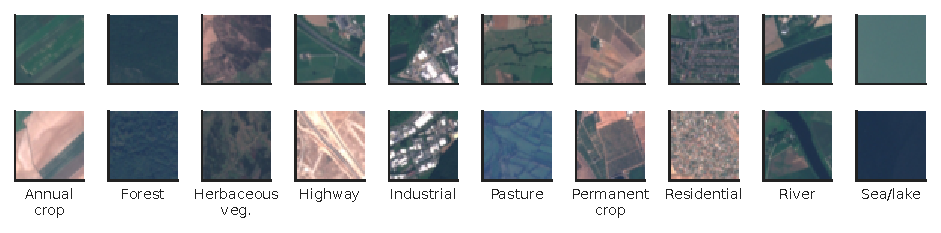
\includegraphics[width=\textwidth,height=0.299\textheight,keepaspectratio]{charts/en/eurosat_samples.pdf}\end{center}\vspace{-3mm}
\chartsource{Source: EuroSAT, Sentinel-2 images (Helber et al., 2019). Data: 27,000 tiles of 64 x 64 pixels, 10 classes.}
\vspace{0.5mm}
\begin{itemize}\setlength{\itemsep}{0pt}
  \item 27\,000 red, green, blue (RGB) tiles of $64\times64$ pixels
    \begin{itemize}\setlength{\itemsep}{0pt}
      \item 2\,000 to 3\,000 per class.
    \end{itemize}
\end{itemize}
\par\vfill\manager{an agricultural lender checks that a farm loan finances crops
    \begin{itemize}\setlength{\itemsep}{0pt}
      \item An insurer maps flood-exposed residential areas.
    \end{itemize}}\par\vspace{0.5mm}
\par\vfill\noindent{\scriptsize\color{FooterGray}(Helber et al., 2019)}\hfill\qlink{NN\_L4\_eurosat\_samples}{Quantlets/L4/NN_L4_eurosat_samples}\par\vspace{0.5mm}
\end{frame}

\begin{frame}{Transfer learning: reuse features learned on a million photos}
\footnotesize
\intuition{the early layers of a network trained on ImageNet detect edges and textures that are useful for any image.}
\begin{columns}[T,onlytextwidth]
\begin{column}{0.53\textwidth}
\[ f_{\btheta}(\mathbf X)=g_{\boldsymbol\psi}\big(\phi_{\boldsymbol\omega}(\mathbf X)\big),\quad \boldsymbol\omega^{(0)}=\boldsymbol\omega_{\mathrm{ImageNet}} \]{\footnotesize\begin{itemize}\setlength{\itemsep}{0pt}
  \item \textbf{\txtwhere}
    \begin{itemize}\setlength{\itemsep}{0pt}
      \item $\phi_{\boldsymbol\omega}$ the convolutional body (512 features after GAP)
      \item $g_{\boldsymbol\psi}$ a new linear head with 10 outputs
    \end{itemize}
\end{itemize}\par}
\end{column}
\begin{column}{0.44\textwidth}
\begin{itemize}\setlength{\itemsep}{2pt}
  \item \textbf{Feature extraction}
    \begin{itemize}\setlength{\itemsep}{0pt}
      \item $\boldsymbol\omega$ frozen; fit only $\boldsymbol\psi$ (here a logistic regression, $C$ chosen on validation)
    \end{itemize}
  \item \textbf{Fine-tuning}
    \begin{itemize}\setlength{\itemsep}{0pt}
      \item All weights trained, smaller learning rate for the body ($3\cdot10^{-4}$) than for the head ($3\cdot10^{-3}$), chosen a priori
    \end{itemize}
  \item \textbf{From scratch}
    \begin{itemize}\setlength{\itemsep}{0pt}
      \item A 4-block CNN, 1\,176\,746 parameters, random start
    \end{itemize}
\end{itemize}
\end{column}
\end{columns}
\par\vfill\manager{feature extraction is the cheapest: one pass over the images and a logistic regression.}\par\vspace{0.5mm}
\par\vfill\noindent{\scriptsize\color{FooterGray}(Yosinski et al., 2014)}\par\vspace{0.5mm}
\end{frame}

\begin{frame}{Experimental protocol for the three transfer strategies}
\footnotesize
\begin{columns}[T,onlytextwidth]
\begin{column}{0.5\textwidth}
\begin{itemize}\setlength{\itemsep}{3pt}
  \item \textbf{Split}, stratified by class
    \begin{itemize}\setlength{\itemsep}{0pt}
      \item 16\,200 train / 5\,400 validation / 5\,400 test tiles
    \end{itemize}
  \item \textbf{Input}
    \begin{itemize}\setlength{\itemsep}{0pt}
      \item Tiles resized to $112\times112$ for ResNet-18, scaled with the ImageNet mean and standard deviation per channel
      \item $\tilde x_c=(x_c-\mu_c)/s_c$
    \end{itemize}
\end{itemize}
\end{column}
\begin{column}{0.47\textwidth}
\begin{itemize}\setlength{\itemsep}{3pt}
  \item \textbf{Training}
    \begin{itemize}\setlength{\itemsep}{0pt}
      \item AdamW, batch 64, one-cycle schedule; flips and $90^\circ$ rotations
      \item From scratch 18 epochs; fine-tuning 6 epochs
      \item Model kept at its best validation accuracy
    \end{itemize}
  \item \textbf{Cost}
    \begin{itemize}\setlength{\itemsep}{0pt}
      \item 1225 seconds for the three main runs on a laptop GPU
    \end{itemize}
\end{itemize}
\end{column}
\end{columns}
\par\vfill\manager{fixing the test tiles before any modelling is what makes the three strategies comparable.}\par\vspace{0.5mm}
\par\vfill\noindent{\scriptsize\color{FooterGray}(own computation)}\hfill\tryit{\S5}\par\vspace{0.5mm}
\end{frame}

\begin{frame}{Fine-tuning is the most accurate, and transfer matters most when labels are few}
\small
\intuition{left: learning with all labels; right: test accuracy when only $n$ labelled tiles per class are available.}
\begin{center}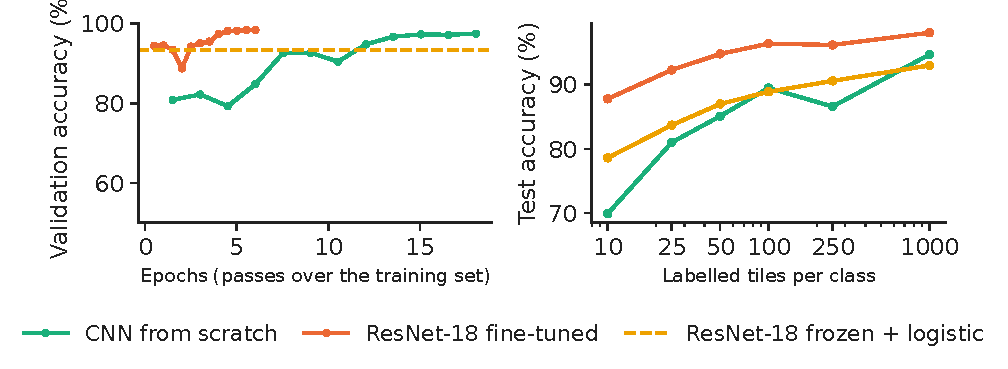
\includegraphics[width=\textwidth,height=0.420\textheight,keepaspectratio]{charts/en/transfer_curves.pdf}\end{center}\vspace{-3mm}
\chartsource{Source: EuroSAT, Sentinel-2 images (Helber et al., 2019). Data: 16,200 training, 5,400 validation, 5,400 test tiles; right: mean of 2 seeds.}
\vspace{0.5mm}
\begin{itemize}\setlength{\itemsep}{0pt}
  \item Test accuracy, all labels: from scratch 97.78\,\%, frozen + logistic 93.48\,\%, fine-tuned 98.76\,\%.
  \item With 10 tiles per class: scratch 69.9\,\%, frozen 78.6\,\%, fine-tuned 87.8\,\%.
\end{itemize}
\par\vfill\noindent{\scriptsize\color{FooterGray}(own computation)}\hfill\qlink{NN\_L4\_transfer\_curves}{Quantlets/L4/NN_L4_transfer_curves}\par\vspace{0.5mm}
\end{frame}

\begin{frame}{The label budget and the savings from transfer learning}
\footnotesize
\begin{columns}[T,onlytextwidth]
\begin{column}{0.47\textwidth}
{\footnotesize\renewcommand{\arraystretch}{1.05}\setlength{\tabcolsep}{4pt}
\begin{tabular}{@{}rrrr@{}}\toprule
Tiles/class & Scratch & Frozen & Fine-tuned \\ \midrule
10 & 69.9 & 78.6 & 87.8 \\
25 & 81.0 & 83.7 & 92.3 \\
50 & 85.1 & 87.0 & 94.8 \\
100 & 89.5 & 88.9 & 96.4 \\
250 & 86.6 & 90.6 & 96.2 \\
1000 & 94.7 & 93.0 & 98.1 \\
\bottomrule\end{tabular}}
\par\vspace{0.5mm}{\scriptsize \begin{itemize}\setlength{\itemsep}{0pt}
  \item Test accuracy (\%), mean of 2 random draws of the labelled tiles; same 5,400 test tiles.
\end{itemize}}
\end{column}
\begin{column}{0.5\textwidth}
\begin{itemize}\setlength{\itemsep}{4pt}
  \item With 100 labelled tiles in total, the pre-trained network already beats a CNN trained from scratch on the same labels by a wide margin.
  \item The scratch CNN needs the full budget to approach the fine-tuned network.
  \item The run of the whole table took 1857 seconds.
\end{itemize}
\end{column}
\end{columns}
\par\vfill\manager{labelling a tile costs an expert's minute
    \begin{itemize}\setlength{\itemsep}{0pt}
      \item Transfer learning turns weeks of labelling into an afternoon.
    \end{itemize}}\par\vspace{0.5mm}
\par\vfill\noindent{\scriptsize\color{FooterGray}(own computation)}\par\vspace{0.5mm}
\end{frame}

\begin{frame}{Remaining errors: annual versus permanent crops}
\small
\intuition{the fine-tuned network mixes classes that look alike from space.}
\begin{center}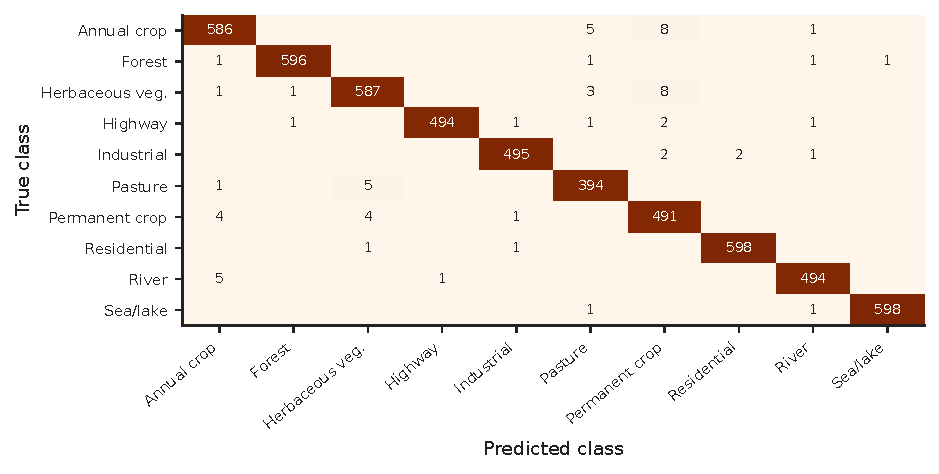
\includegraphics[width=\textwidth,height=0.500\textheight,keepaspectratio]{charts/en/eurosat_confusion.pdf}\end{center}\vspace{-3mm}
\chartsource{Source: EuroSAT, Sentinel-2 images (Helber et al., 2019). Data: 5,400 test tiles, fine-tuned ResNet-18, seed 20261108.}
\vspace{0.5mm}
\begin{itemize}\setlength{\itemsep}{0pt}
  \item 67 errors on 5\,400 tiles
    \begin{itemize}\setlength{\itemsep}{0pt}
      \item Largest: Annual crop taken for Permanent crop (8)
      \item Macro-F1 98.72\,\%.
    \end{itemize}
\end{itemize}
\par\vfill\noindent{\scriptsize\color{FooterGray}(own computation)}\hfill\qlink{NN\_L4\_eurosat\_confusion}{Quantlets/L4/NN_L4_eurosat_confusion}\par\vspace{0.5mm}
\end{frame}

\begin{frame}{Grad-CAM: image regions behind the classification}
\footnotesize
\intuition{weight each feature map by how much the class score reacts to it, sum, and keep the positive part.}
\begin{columns}[T,onlytextwidth]
\begin{column}{0.46\textwidth}
\[ \alpha^{c}_o=\frac{1}{HW}\sum_{i,j}\frac{\partial z_c}{\partial A_o(i,j)} \]\vspace{-2mm}\[ M^{c}=\ReLU\Big(\sum_o\alpha^{c}_oA_o\Big) \]{\footnotesize\begin{itemize}\setlength{\itemsep}{0pt}
  \item \textbf{\txtwhere}
    \begin{itemize}\setlength{\itemsep}{0pt}
      \item $z_c$ the score (logit) of class $c$
      \item $A_o$ feature map $o$ of the chosen layer
      \item $M^c$ the class activation map (CAM), upsampled to the tile
    \end{itemize}
\end{itemize}\par}
\end{column}
\begin{column}{0.51\textwidth}
\begin{center}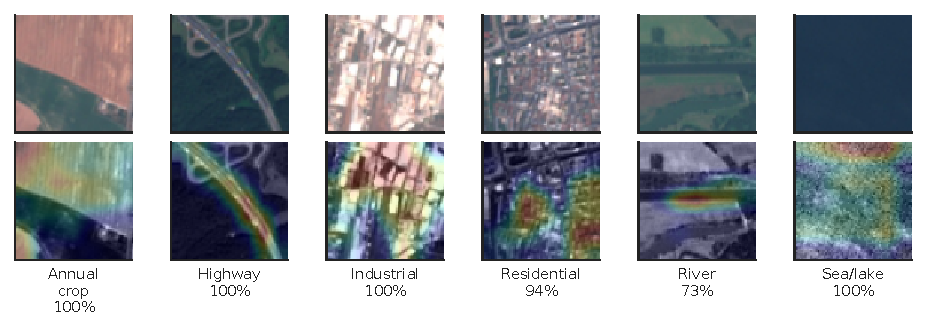
\includegraphics[width=\textwidth,height=0.550\textheight,keepaspectratio]{charts/en/gradcam.pdf}\end{center}\vspace{-3mm}
\chartsource{Source: EuroSAT, Sentinel-2 images (Helber et al., 2019). Data: six test tiles; Grad-CAM on the 7 x 7 maps of block 3 of the fine-tuned ResNet-18.}
\end{column}
\end{columns}
\par\vfill\manager{an auditor can check that ``industrial'' is decided by the roofs, not by a cloud or a border artefact.}\par\vspace{0.5mm}
\par\vfill\noindent{\scriptsize\color{FooterGray}(Selvaraju et al., 2017; own computation)}\hfill\qlink{NN\_L4\_gradcam}{Quantlets/L4/NN_L4_gradcam}\par\vspace{0.5mm}
\end{frame}

\begin{frame}{From tiles to a decision: land-use shares}
\footnotesize
\intuition{a portfolio question is about shares and totals, so errors that cancel matter less than errors that do not.}
\begin{columns}[T,onlytextwidth]
\begin{column}{0.53\textwidth}
\[ \hat\pi_k=\frac1n\sum_{i=1}^n\mathbf 1\{\hat y_i=k\},\qquad \E[\hat\pi_k]=\sum_j\pi_j\,P(\hat y=k\mid y=j) \]{\footnotesize\begin{itemize}\setlength{\itemsep}{0pt}
  \item \textbf{\txtwhere}
    \begin{itemize}\setlength{\itemsep}{0pt}
      \item $\pi_k$ true share of class $k$ in a region
      \item $P(\hat y=k\mid y=j)$ the confusion matrix, estimated on the test tiles
    \end{itemize}
\end{itemize}\par}
\end{column}
\begin{column}{0.44\textwidth}
\begin{itemize}\setlength{\itemsep}{2pt}
  \item Test tiles: share of crops (annual + permanent) 20.37\,\% true vs 20.54\,\% predicted.
  \item Largest error of any class share: 0.20 percentage points.
  \item Inverting the confusion matrix corrects the shares when the error rates are stable (domain shift breaks this).
\end{itemize}
\end{column}
\end{columns}
\par\vfill\manager{for an insurer or an agricultural lender the output is a share of hectares per region, with an error bar, not a label per tile.}\par\vspace{0.5mm}
\par\vfill\noindent{\scriptsize\color{FooterGray}(own computation)}\par\vspace{0.5mm}
\end{frame}

\begin{frame}{When transfer learning helps, and when it can mislead}
\footnotesize
\begin{columns}[T,onlytextwidth]
\begin{column}{0.49\textwidth}
\begin{itemize}\setlength{\itemsep}{4pt}
  \item \textbf{Helps most}
    \begin{itemize}\setlength{\itemsep}{0pt}
      \item Few labels (right panel of the transfer chart)
      \item A source domain with similar low-level statistics (edges, textures)
      \item A limited compute budget: frozen features cost one forward pass
    \end{itemize}
\end{itemize}
\end{column}
\begin{column}{0.48\textwidth}
\begin{itemize}\setlength{\itemsep}{4pt}
  \item \textbf{Can mislead}
    \begin{itemize}\setlength{\itemsep}{0pt}
      \item Domain shift: other season, other sensor, other country than the training tiles
      \item Spurious cues learned from the source (watermarks, borders)
      \item The test set must come from the population where the model will be used
    \end{itemize}
\end{itemize}
\end{column}
\end{columns}
\par\vfill\manager{before deployment, label a small sample from the target region and re-measure
    \begin{itemize}\setlength{\itemsep}{0pt}
      \item The fine-tuned model is cheap to update.
    \end{itemize}}\par\vspace{0.5mm}
\par\vfill\noindent{\scriptsize\color{FooterGray}(Yosinski et al., 2014; Helber et al., 2019)}\par\vspace{0.5mm}
\end{frame}

\begin{frame}{Convolutions beyond photos: sequences and charts}
\footnotesize
\intuition{a one-dimensional convolution slides over time, the same way a two-dimensional one slides over space.}
\begin{columns}[T,onlytextwidth]
\begin{column}{0.53\textwidth}
\[ z_t=b+\sum_{c}\sum_{u=0}^{k-1}K_c(u)\,x_{c,\,t-u} \]{\footnotesize\begin{itemize}\setlength{\itemsep}{0pt}
  \item \textbf{\txtwhere}
    \begin{itemize}\setlength{\itemsep}{0pt}
      \item $x_{c,t}$ input series $c$ at time $t$ (returns, volume, load)
      \item Causal: only past values
    \end{itemize}
\end{itemize}\par}
\end{column}
\begin{column}{0.44\textwidth}
\begin{itemize}\setlength{\itemsep}{2pt}
  \item A one-dimensional CNN is a learned bank of moving-average filters
    \begin{itemize}\setlength{\itemsep}{0pt}
      \item Lecture 5 compares it with recurrent networks.
    \end{itemize}
  \item Charts of markets can be read as images by a vision--language model (VLM): research of our group, next section.
  \item Same rules: real data, a time-ordered split, a simple benchmark first.
\end{itemize}
\end{column}
\end{columns}
\par\vfill\manager{a risk desk can screen hundreds of chart panels per day with a model, and keep the analyst for the flagged ones.}\par\vspace{0.5mm}
\par\vfill\noindent{\scriptsize\color{FooterGray}(Bishop \& Bishop, 2024, ch.~10)}\par\vspace{0.5mm}
\end{frame}

\section*{Wrap-up}

\begin{frame}{Quiz 1: output size}
\small
\begin{itemize}
  \item A $64\times64$ tile passes a $3\times3$ convolution with padding 1 and stride 2
    \begin{itemize}\setlength{\itemsep}{0pt}
      \item How large is the output map?
    \end{itemize}
\end{itemize}
\vspace{2mm}
\begin{exampleblock}{Answer}
\begin{itemize}
  \item $\lfloor(64+2-3)/2\rfloor+1=32$, so $32\times32$.
\end{itemize}
\end{exampleblock}
\end{frame}

\begin{frame}{Quiz 2: parameters}
\small
\begin{itemize}
  \item Why does our CNN beat the MLP on Fashion-MNIST with fewer parameters?
\end{itemize}
\vspace{2mm}
\begin{exampleblock}{Answer}
\begin{itemize}
  \item Weight sharing and local connectivity encode the structure of images
    \begin{itemize}\setlength{\itemsep}{0pt}
      \item The CNN reaches 93.08\,\% with 140\,778 parameters against 89.00\,\% with 235\,146.
    \end{itemize}
\end{itemize}
\end{exampleblock}
\end{frame}

\begin{frame}{Quiz 3: depth}
\small
\begin{itemize}
  \item A plain 32-layer network has a higher training loss than a residual one of the same depth
    \begin{itemize}\setlength{\itemsep}{0pt}
      \item Is that overfitting?
    \end{itemize}
\end{itemize}
\vspace{2mm}
\begin{exampleblock}{Answer}
\begin{itemize}
  \item No: overfitting lowers the training loss
    \begin{itemize}\setlength{\itemsep}{0pt}
      \item This is the degradation problem (0.557 vs 0.291), solved by the identity shortcut.
    \end{itemize}
\end{itemize}
\end{exampleblock}
\end{frame}

\begin{frame}{Quiz 4: a label budget}
\small
\begin{itemize}
  \item You can label only 100 satellite tiles in total
    \begin{itemize}\setlength{\itemsep}{0pt}
      \item Which strategy do you choose?
    \end{itemize}
\end{itemize}
\vspace{2mm}
\begin{exampleblock}{Answer}
\begin{itemize}
  \item A pre-trained network: with 10 tiles per class, fine-tuning gives 87.8\,\% and frozen features 78.6\,\%, against 69.9\,\% from scratch.
\end{itemize}
\end{exampleblock}
\end{frame}

\begin{frame}{Quiz 5: explanation}
\small
\begin{itemize}
  \item A Grad-CAM map of an ``industrial'' tile lights up a cloud
    \begin{itemize}\setlength{\itemsep}{0pt}
      \item What do you do?
    \end{itemize}
\end{itemize}
\vspace{2mm}
\begin{exampleblock}{Answer}
\begin{itemize}
  \item Treat it as a warning of a spurious cue: inspect similar tiles, add cloudy examples or a cloud mask, and re-test on the target region.
\end{itemize}
\end{exampleblock}
\end{frame}

\begin{frame}{Wrap-up}
\small
\vspace{-2mm}\begin{multicols}{2}\scriptsize\tableofcontents\end{multicols}
\begin{itemize}\setlength{\itemsep}{1pt}
  \item A convolution is a shared local filter
    \begin{itemize}\setlength{\itemsep}{0pt}
      \item Padding, stride and pooling set the map size, depth and pooling the receptive field.
    \end{itemize}
  \item On real images the CNN beats the MLP with fewer parameters
    \begin{itemize}\setlength{\itemsep}{0pt}
      \item Residual blocks make depth trainable
      \item Augmentation is free data.
    \end{itemize}
  \item Transfer learning wins when labels are scarce.
    \begin{itemize}\setlength{\itemsep}{0pt}
      \item Next: sequences and recurrent networks (Lecture 5).
    \end{itemize}
\end{itemize}
\end{frame}

\begin{frame}{Research from our group: vision models for finance}
\footnotesize
\begin{itemize}\setlength{\itemsep}{4pt}
  \item \textbf{A multimodal vision--language framework for financial anomaly detection} (Jheng, Pele, Tak \& Găman, 2026, PICBE), Best Paper Award at the International Conference on Business Excellence (ICBE) 2026
    \begin{itemize}\setlength{\itemsep}{0pt}
      \item Market indicators projected onto a standardised multi-panel image; market regime classification treated as visual recognition
      \item Zero-shot vision--language model (GPT-4.1, a generative pre-trained transformer) with rolling-quantile labels and structured natural-language rationales
      \item Out-of-sample tests on the S\&P 500: promising fidelity in detecting systemic anomalies, with interpretable explanations
    \end{itemize}
  \item \textbf{Quantlet: the code snippet knowledge platform} (Găman, Winkel, Zuo, Härdle \& Pele, 2026, Computational Statistics)
    \begin{itemize}\setlength{\itemsep}{0pt}
      \item The platform on which every chart of this lecture is published as a reproducible Quantlet
    \end{itemize}
\end{itemize}
\par\vspace{0.5mm}{\scriptsize \begin{itemize}\setlength{\itemsep}{0pt}
  \item Findings as stated in the papers; numbers on the other slides come from our own computations.
\end{itemize}}
\par\vfill\noindent{\scriptsize\color{FooterGray}(Bucharest University of Economic Studies; Romanian Academy, Institute for Economic Forecasting)}\par\vspace{0.5mm}
\end{frame}

\begin{frame}{Further reading and resources}
\small
\begin{columns}[T,onlytextwidth]
\begin{column}{0.52\textwidth}
\begin{itemize}\setlength{\itemsep}{4pt}
  \item \textbf{Bishop \& Bishop (2024)}, ch.~10: convolutional networks, with the derivations of this lecture.
  \item \textbf{Goodfellow, Bengio \& Courville (2016)}, ch.~9: convolution, pooling, variants.
  \item \textbf{He et al. (2016)}: the ResNet paper, short and readable.
\end{itemize}
\end{column}
\begin{column}{0.45\textwidth}
\begin{itemize}\setlength{\itemsep}{4pt}
  \item \textbf{This course}: code, data, notebooks --- \href{https://github.com/danpele/NEURAL_BIZ}{github.com/danpele/NEURAL\_BIZ}.
  \item \textbf{Experiment yourself}: the notebook reproduces the charts of this lecture --- \href{\nnrepo/\nnnb}{notebooks/}.
  \item \textbf{Seminar 4}: transfer learning on EuroSAT with your own label budget.
\end{itemize}
\end{column}
\end{columns}
\end{frame}

\begin{frame}{References (1/2)}
\scriptsize
\begin{itemize}\setlength{\itemsep}{0pt}\scriptsize
\item Bishop, C.\,M.\ \& Bishop, H.\ (2024). \textit{Deep Learning: Foundations and Concepts}, ch.~10. Springer. \href{https://doi.org/10.1007/978-3-031-45468-4}{doi:10.1007/978-3-031-45468-4}
\item Goodfellow, I., Bengio, Y.\ \& Courville, A.\ (2016). \textit{Deep Learning}, ch.~9. MIT Press. \href{https://www.deeplearningbook.org}{deeplearningbook.org}
\item He, K., Zhang, X., Ren, S.\ \& Sun, J.\ (2016). Deep residual learning for image recognition. \textit{CVPR}, 770--778. \href{https://doi.org/10.1109/CVPR.2016.90}{doi:10.1109/CVPR.2016.90}
\item Helber, P., Bischke, B., Dengel, A.\ \& Borth, D.\ (2019). EuroSAT: A novel dataset and deep learning benchmark for land use and land cover classification. \textit{IEEE JSTARS}, 12(7), 2217--2226. \href{https://doi.org/10.1109/JSTARS.2019.2918242}{doi:10.1109/JSTARS.2019.2918242}
\item Ioffe, S.\ \& Szegedy, C.\ (2015). Batch normalization: Accelerating deep network training by reducing internal covariate shift. \textit{ICML}, PMLR 37, 448--456. \href{https://arxiv.org/abs/1502.03167}{arXiv:1502.03167}
\item Jheng, S.-L., Pele, D.\,T., Tak, R.\ \& Găman, Ș.\ (2026). A multimodal vision-language framework for financial anomaly detection. \textit{Proceedings of the International Conference on Business Excellence}, 20(1), 191--201. \href{https://doi.org/10.2478/picbe-2026-0020}{doi:10.2478/picbe-2026-0020}
\item Găman, Ș., Winkel, J., Zuo, X., Härdle, W.\,K.\ \& Pele, D.\,T.\ (2026). Quantlet: the code snippet knowledge platform. \textit{Computational Statistics}, 41(3), 66. \href{https://doi.org/10.1007/s00180-026-01742-6}{doi:10.1007/s00180-026-01742-6}
\item Krizhevsky, A.\ (2009). Learning multiple layers of features from tiny images. Technical report, University of Toronto. \href{https://www.cs.toronto.edu/~kriz/learning-features-2009-TR.pdf}{cs.toronto.edu}
\item Krizhevsky, A., Sutskever, I.\ \& Hinton, G.\,E.\ (2012). ImageNet classification with deep convolutional neural networks. \textit{NIPS}, 25, 1097--1105. \href{https://doi.org/10.1145/3065386}{doi:10.1145/3065386}
\end{itemize}
\end{frame}

\begin{frame}{References (2/2)}
\scriptsize
\begin{itemize}\setlength{\itemsep}{0pt}\scriptsize
\item LeCun, Y., Bottou, L., Bengio, Y.\ \& Haffner, P.\ (1998). Gradient-based learning applied to document recognition. \textit{Proceedings of the IEEE}, 86(11), 2278--2324. \href{https://doi.org/10.1109/5.726791}{doi:10.1109/5.726791}
\item McNemar, Q.\ (1947). Note on the sampling error of the difference between correlated proportions or percentages. \textit{Psychometrika}, 12(2), 153--157. \href{https://doi.org/10.1007/BF02295996}{doi:10.1007/BF02295996}
\item Selvaraju, R.\,R., Cogswell, M., Das, A., Vedantam, R., Parikh, D.\ \& Batra, D.\ (2017). Grad-CAM: Visual explanations from deep networks via gradient-based localization. \textit{ICCV}, 618--626. \href{https://doi.org/10.1109/ICCV.2017.74}{doi:10.1109/ICCV.2017.74}
\item Simonyan, K.\ \& Zisserman, A.\ (2015). Very deep convolutional networks for large-scale image recognition. \textit{ICLR}. \href{https://arxiv.org/abs/1409.1556}{arXiv:1409.1556}
\item Xiao, H., Rasul, K.\ \& Vollgraf, R.\ (2017). Fashion-MNIST: A novel image dataset for benchmarking machine learning algorithms. \href{https://arxiv.org/abs/1708.07747}{arXiv:1708.07747}
\item Yosinski, J., Clune, J., Bengio, Y.\ \& Lipson, H.\ (2014). How transferable are features in deep neural networks? \textit{NIPS}, 27, 3320--3328. \href{https://arxiv.org/abs/1411.1792}{arXiv:1411.1792}
\item Zeiler, M.\,D.\ \& Fergus, R.\ (2014). Visualizing and understanding convolutional networks. \textit{ECCV}, 818--833. \href{https://doi.org/10.1007/978-3-319-10590-1_53}{doi:10.1007/978-3-319-10590-1\_53}
\end{itemize}
\end{frame}

\appendix

\begin{frame}{Appendix: convolution as a matrix product}
\footnotesize
\begin{itemize}\setlength{\itemsep}{3pt}
  \item Stack every $k\times k\times C_{\mathrm{in}}$ patch of the input as a row of $\mathbf P\in\R^{H_{\mathrm{out}}W_{\mathrm{out}}\times k^2C_{\mathrm{in}}}$ (``im2col'').
  \item Stack the kernels as columns of $\mathbf K\in\R^{k^2C_{\mathrm{in}}\times C_{\mathrm{out}}}$
    \begin{itemize}\setlength{\itemsep}{0pt}
      \item Then $\mathbf Z=\mathbf P\mathbf K+\mathbf 1\vb^{\top}$.
    \end{itemize}
  \item Gradients follow from the matrix rules of Lecture 2: $\partial\loss/\partial\mathbf K=\mathbf P^{\top}\boldsymbol\Delta$ and $\partial\loss/\partial\mathbf P=\boldsymbol\Delta\mathbf K^{\top}$, with $\boldsymbol\Delta=\partial\loss/\partial\mathbf Z$.
  \item Adding back the rows of $\partial\loss/\partial\mathbf P$ to their pixel positions (``col2im'') gives $\partial\loss/\partial\mathbf X$: the full convolution of the main text.
  \item A $1\times1$ convolution is the special case $k=1$: a dense layer applied to the channels of every pixel.
\end{itemize}
\end{frame}

\begin{frame}{Appendix: the CNN of the case study in PyTorch}
\footnotesize
{\scriptsize\ttfamily\setlength{\parindent}{0pt}block = lambda a, b: [nn.Conv2d(a, b, 3, padding=1), nn.BatchNorm2d(b), nn.ReLU()]\\
cnn = nn.Sequential(*block(1, 32), *block(32, 32), nn.MaxPool2d(2),\ \ \ \  \# 28 -> 14\\
\hspace*{10.0em}*block(32, 64), *block(64, 64), nn.MaxPool2d(2),\ \ \ \ \# 14 -> 7\\
\hspace*{10.0em}*block(64, 128), nn.AdaptiveAvgPool2d(1), nn.Flatten(),\\
\hspace*{10.0em}nn.Dropout(0.3), nn.Linear(128, 10))\\
resnet = torchvision.models.resnet18(weights='IMAGENET1K\_V1')\\
resnet.fc = nn.Linear(512, 10)\ \ \ \ \ \ \ \ \ \ \ \ \ \ \ \ \# new head for the 10 land-use classes\par}\begin{itemize}\setlength{\itemsep}{2pt}
  \item Full code: lectures/L4/analysis\_L4.py and the notebook of this lecture.
\end{itemize}
\end{frame}

\end{document}
